% !TeX root = ../main.tex

%%% Tables %%%

\begin{table}[h]
\centering
\caption{Accuracies and run times for all models. All reported values are averages, and $\pm$ refers to the standard deviation. The run times heavily depend upon the optimization method.}
\begin{tabular}{ccccccc}
Model       & \multicolumn{1}{c}{Training Time (Minutes)} & \multicolumn{1}{c}{Dive Accuracy} & \multicolumn{1}{c}{Subdive Accuracy}  \\ \hline
CarHMM-DFT  & $61.68 \pm 10.21$                            & -------------                     & $1.00 \pm 0.00$                       \\ 
HHMM-DFT    & $139.76 \pm 28.93$                           & $0.94 \pm 0.03$                   & $1.00 \pm 0.00$                       \\
CarHHMM     & $257.58 \pm 81.64$                           & $0.87 \pm 0.11$                   & $0.89 \pm 0.01$                       \\
CarHHMM-DFT & $150.18 \pm 36.94$                           & $0.94 \pm 0.02$                   & $1.00 \pm 0.00$                       \\
\end{tabular}
\label{table:accuracy}
\end{table}

\begin{table}[ht]
    \centering
    \caption{Estimates and standard errors of emission parameters for killer whale data under the CarHHMM-DFT.}
    \scalebox{0.8}{
\begin{tabular}{ccccc}
    \multirow{2}{*}{Feature}                                                       & \multirow{2}{*}{Dive / Subdive Type} & \multicolumn{3}{c}{Parameter Estimate}              \\
                                                                                   &                                      & $\hat \mu$      & $\hat \sigma$   & $\hat \phi$     \\ \hline
    \multirow{2}{*}{Dive Duration $(s)$ - $Y$}                                     & 1                                    & $25.687 \pm 0.602$ & $9.573 \pm 0.514$ & ---             \\
                                                                                   & 2                                    & $104.601 \pm 9.395$ & $64.678 \pm 7.468$ & ---             \\ \hline
    \multirow{3}{*}{x-acceleration $(m/s^2)$ - $\left(\mathbf{Z}^{*(1)}\right)_x$} & 1                                    & $0.020 \pm 0.042$ & $0.034 \pm 0.001$ & $0.976 \pm 0.007$ \\
                                                                                   & 2                                    & $0.244 \pm 0.013$ & $0.079 \pm 0.001$ & $0.886 \pm 0.005$ \\
                                                                                   & 3                                    & $0.218 \pm 0.028$ & $0.265 \pm 0.007$ & $0.626 \pm 0.029$ \\ \hline
    \multirow{3}{*}{y-acceleration $(m/s^2)$ - $\left(\mathbf{Z}^{*(1)}\right)_y$} & 1                                    & $0.469 \pm 0.052$ & $0.044 \pm 0.001$ & $0.976 \pm 0.009$ \\
                                                                                   & 2                                    & $0.436 \pm 0.014$ & $0.082 \pm 0.001$ & $0.886 \pm 0.012$ \\
                                                                                   & 3                                    & $0.384 \pm 0.033$ & $0.321 \pm 0.009$ & $0.626 \pm 0.034$ \\ \hline
    \multirow{3}{*}{z-acceleration $(m/s^2)$ - $\left(\mathbf{Z}^{*(1)}\right)_z$} & 1                                    & $-0.683 \pm 0.061$ & $0.052 \pm 0.001$ & $0.976 \pm 0.005$ \\
                                                                                   & 2                                    & $-0.593 \pm 0.016$ & $0.096 \pm 0.001$ & $0.886 \pm 0.009$ \\
                                                                                   & 3                                    & $-0.366 \pm 0.033$ & $0.317 \pm 0.009$ & $0.626 \pm 0.033$ \\ \hline
    \multirow{3}{*}{Fourier sum - $Z^{*(2)}$}                                      & 1                                    & $23.340 \pm 0.282$ & $12.948 \pm 0.269$ & ---             \\
                                                                                   & 2                                    & $301.189 \pm 3.244$ & $330.050 \pm 4.166$ & ---             \\
                                                                                   & 3                                    & $10204.010 \pm 211.242$ & $15299.066 \pm 352.674$ & ---             \\ \hline
    \end{tabular}
    }
    \label{table:emis_dists_CarHHMM-DFT}
\end{table}

\begin{table}[ht]
\centering
\label{table:emis_dists_CarHHMM}
\caption{Estimates and standard errors of parameters for killer whale data under the CarHHMM.}
\scalebox{0.8}{
    \begin{tabular}{ccccc}
    \multirow{2}{*}{Feature}                                                       & \multirow{2}{*}{Dive / Subdive Type} & \multicolumn{3}{c}{Parameter Estimate}              \\
                                                                                   &                                      & $\hat \mu$      & $\hat \sigma$   & $\hat \phi$     \\ \hline
    \multirow{2}{*}{Dive Duration $(s)$ - $Y$}                                     & 1                                    & $27.214 \pm 0.667$ & $11.635 \pm 0.699$ & ---             \\
                                                                                   & 2                                    & $135.575 \pm 11.330$ & $63.849 \pm 9.414$ & ---             \\ \hline
    \multirow{3}{*}{x-acceleration $(m/s^2)$ - $\left(\mathbf{Z}^{*(1)}\right)_x$} & 1                                    & $-0.061 \pm 0.088$ & $0.392 \pm 0.019$ & $0.725 \pm 0.045$ \\
                                                                                   & 2                                    & $0.228 \pm 0.017$ & $0.043 \pm 0.001$ & $0.945 \pm 0.004$ \\
                                                                                   & 3                                    & $0.172 \pm 0.012$ & $0.129 \pm 0.003$ & $0.721 \pm 0.017$ \\ \hline
    \multirow{3}{*}{y-acceleration $(m/s^2)$ - $\left(\mathbf{Z}^{*(1)}\right)_y$} & 1                                    & $0.375 \pm 0.122$ & $0.552 \pm 0.033$ & $0.725 \pm 0.064$ \\
                                                                                   & 2                                    & $0.387 \pm 0.020$ & $0.052 \pm 0.001$ & $0.945 \pm 0.011$ \\
                                                                                   & 3                                    & $0.441 \pm 0.011$ & $0.118 \pm 0.002$ & $0.721 \pm 0.023$ \\ \hline
    \multirow{3}{*}{z-acceleration $(m/s^2)$ - $\left(\mathbf{Z}^{*(1)}\right)_z$} & 1                                    & $-0.435 \pm 0.112$ & $0.506 \pm 0.028$ & $0.725 \pm 0.055$ \\
                                                                                   & 2                                    & $-0.537 \pm 0.023$ & $0.059 \pm 0.001$ & $0.945 \pm 0.008$ \\
                                                                                   & 3                                    & $-0.561 \pm 0.012$ & $0.135 \pm 0.003$ & $0.721 \pm 0.018$ \\ \hline
    \end{tabular}
}
\end{table}


\begin{table}[ht]
\centering
\label{table:emis_dists_HHMM}
\caption{Estimates and standard errors of parameters for killer whale data under the HHMM.}
\scalebox{0.8}{
    \begin{tabular}{ccccc}
    \multirow{2}{*}{Feature}                                                       & \multirow{2}{*}{Dive / Subdive Type} & \multicolumn{3}{c}{Parameter Estimate}              \\
                                                                                   &                                      & $\hat \mu$      & $\hat \sigma$   & $\hat \phi$     \\ \hline
    \multirow{2}{*}{Dive Duration $(s)$ - $Y$}                                     & 1                                    & $25.339 \pm 0.599$ & $8.824 \pm 0.511$ & ---             \\
                                                                                   & 2                                    & $92.748 \pm 7.733$ & $63.714 \pm 6.536$ & ---             \\ \hline
    \multirow{3}{*}{x-acceleration $(m/s^2)$ - $\left(\mathbf{Z}^{*(1)}\right)_x$} & 1                                    & $-0.023 \pm 0.002$ & $0.053 \pm 0.001$ & ---             \\
                                                                                   & 2                                    & $0.074 \pm 0.003$ & $0.149 \pm 0.002$ & ---             \\
                                                                                   & 3                                    & $0.214 \pm 0.014$ & $0.422 \pm 0.010$ & ---             \\ \hline
    \multirow{3}{*}{y-acceleration $(m/s^2)$ - $\left(\mathbf{Z}^{*(1)}\right)_y$} & 1                                    & $0.342 \pm 0.002$ & $0.064 \pm 0.002$ & ---             \\
                                                                                   & 2                                    & $0.408 \pm 0.002$ & $0.091 \pm 0.001$ & ---             \\
                                                                                   & 3                                    & $0.320 \pm 0.011$ & $0.341 \pm 0.008$ & ---             \\ \hline
    \multirow{3}{*}{z-acceleration $(m/s^2)$ - $\left(\mathbf{Z}^{*(1)}\right)_z$} & 1                                    & $-0.418 \pm 0.003$ & $0.104 \pm 0.002$ & ---             \\
                                                                                   & 2                                    & $-0.478 \pm 0.003$ & $0.136 \pm 0.002$ & ---             \\
                                                                                   & 3                                    & $-0.346 \pm 0.012$ & $0.359 \pm 0.008$ & ---             \\ \hline
    \multirow{3}{*}{Fourier sum - $Z^{*(2)}$}                                      & 1                                    & $25.321 \pm 0.379$ & $15.938 \pm 0.382$ & ---             \\
                                                                                   & 2                                    & $252.403 \pm 2.786$ & $296.901 \pm 3.910$ & ---             \\
                                                                                   & 3                                    & $8798.207 \pm 149.370$ & $15579.337 \pm 286.878$ & ---             \\ \hline
    \end{tabular}
}
\end{table}




%%% model definitions %%%

\begin{figure}[ht]
    \begin{subfigure}{\textwidth}
      \centering
      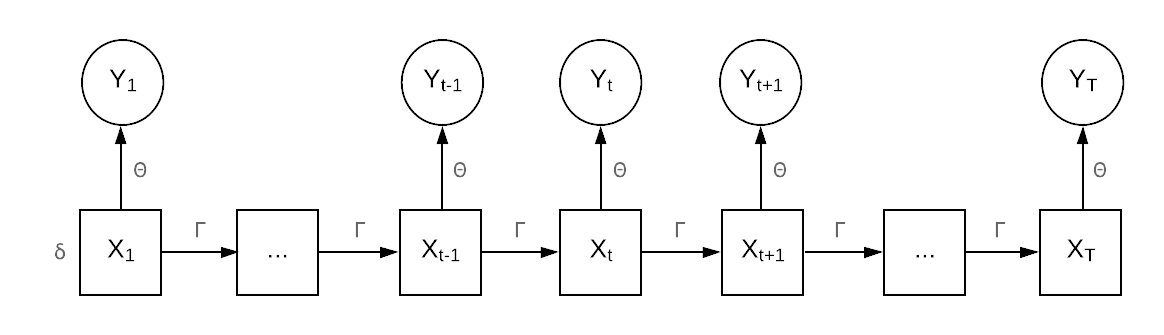
\includegraphics[width=4in]{../Plots/HMM.png}  
      \caption{Hidden Markov Model (\textbf{HMM})}
      \label{fig:HMM}
    \end{subfigure}
    %
    \newline
    %
    \begin{subfigure}{\textwidth}
      \centering
      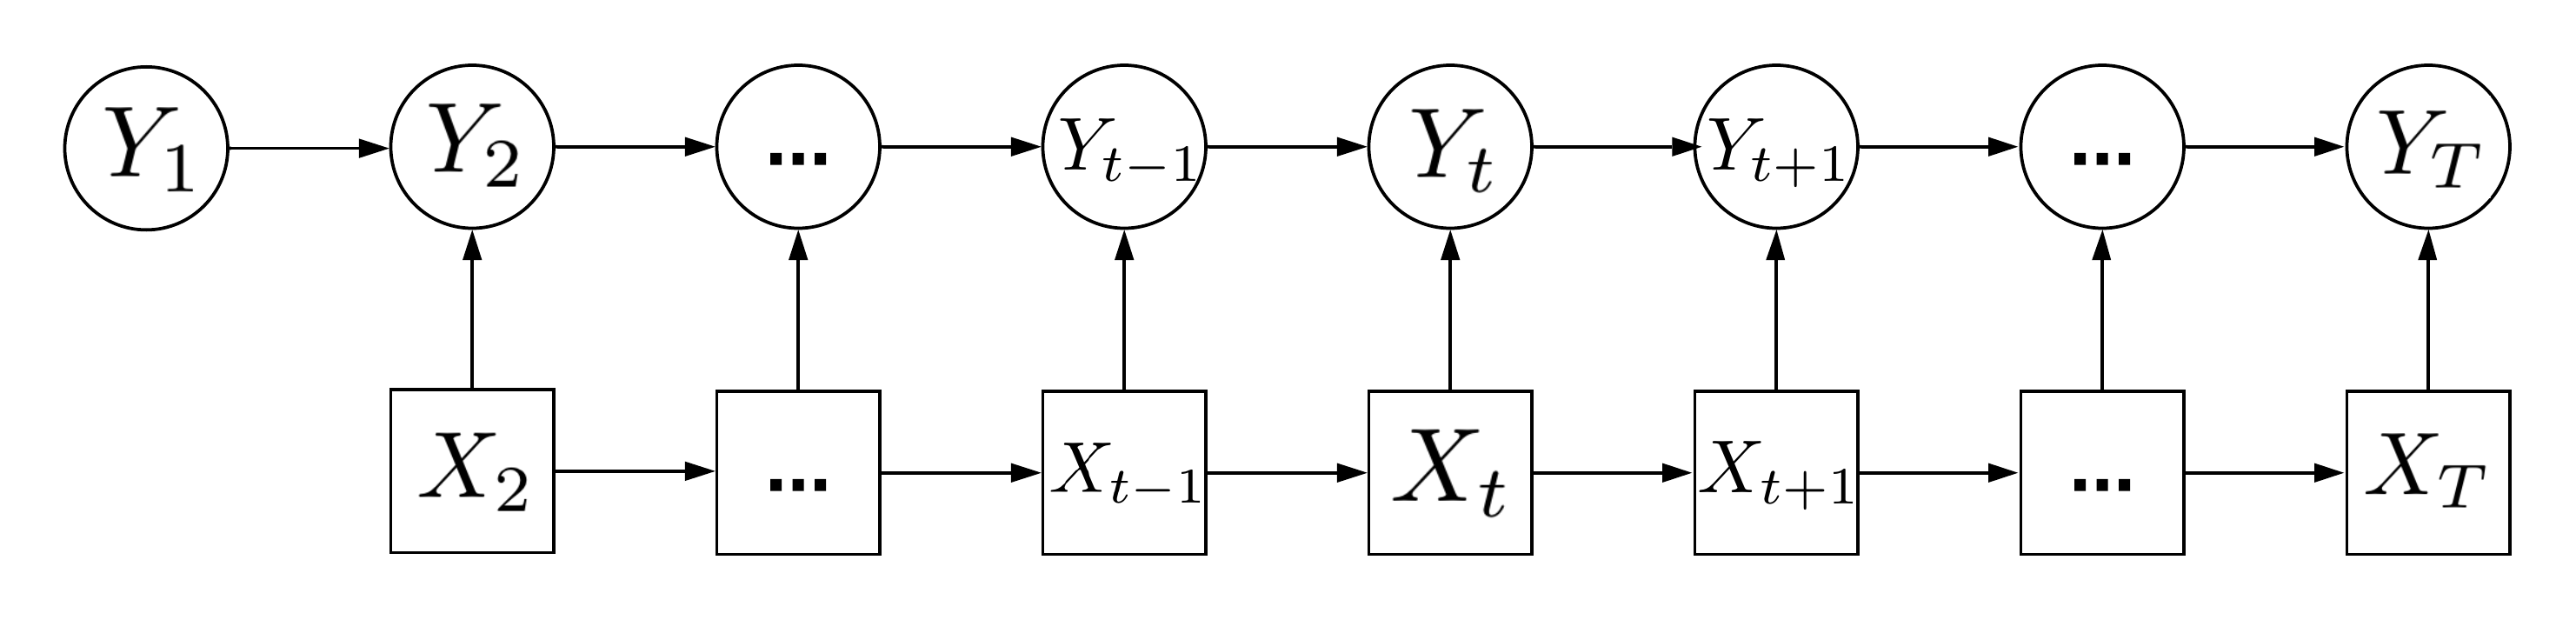
\includegraphics[width=4in]{../Plots/CarHMM.png}  
      \caption{Conditionally Auto-regressive HMM (\textbf{CarHMM})}
      \label{fig:CarHMM}
    \end{subfigure}
    %
    \newline
    %
    \begin{subfigure}{\textwidth}
      \centering
      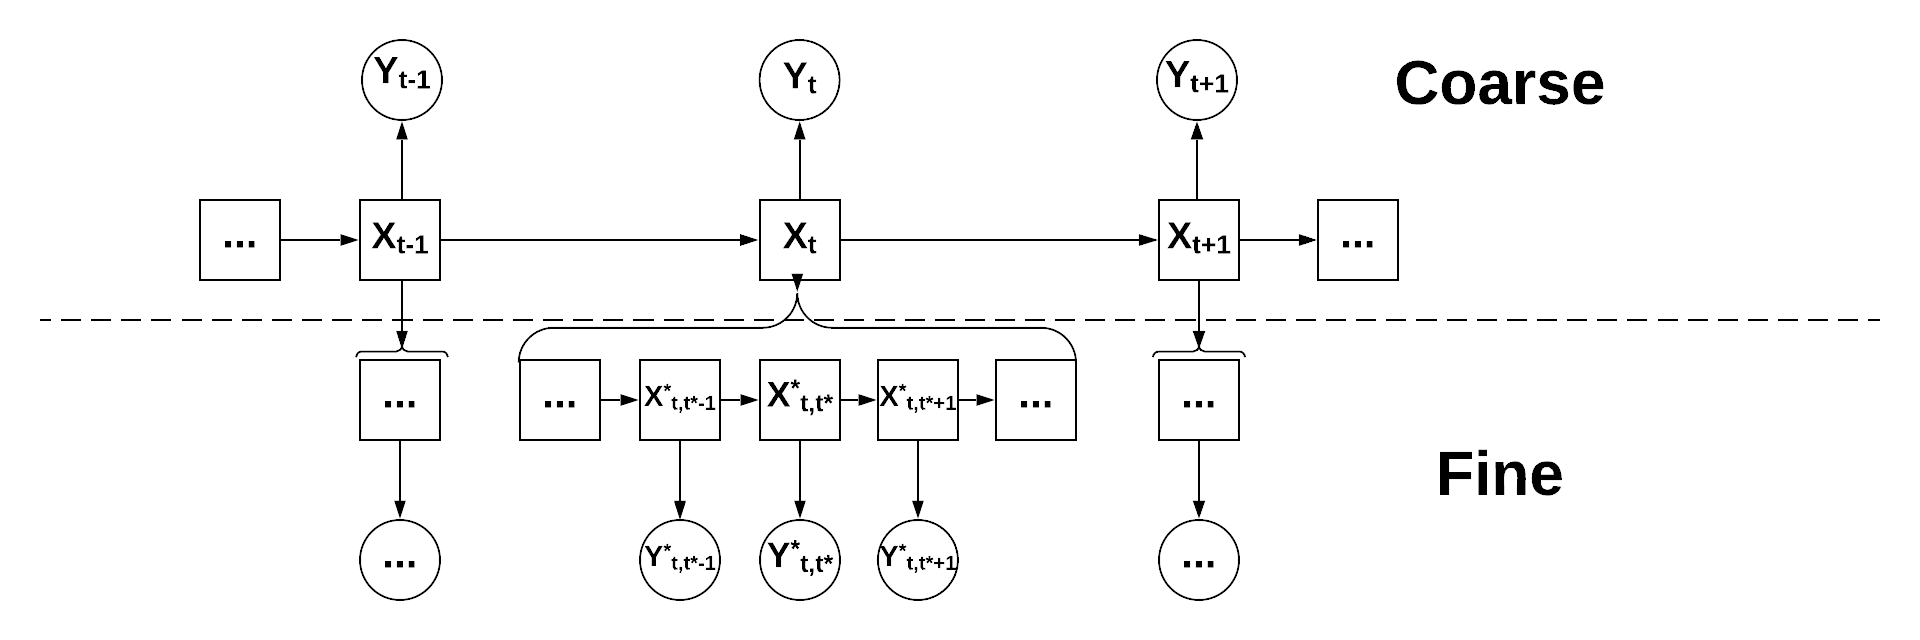
\includegraphics[width=4in]{../Plots/HHMM.png}  
      \caption{Hierarchical HMM (\textbf{HHMM})}
      \label{fig:HHMM}
    \end{subfigure}
    %
    \newline
    %
    \begin{subfigure}{\textwidth}
      \centering
      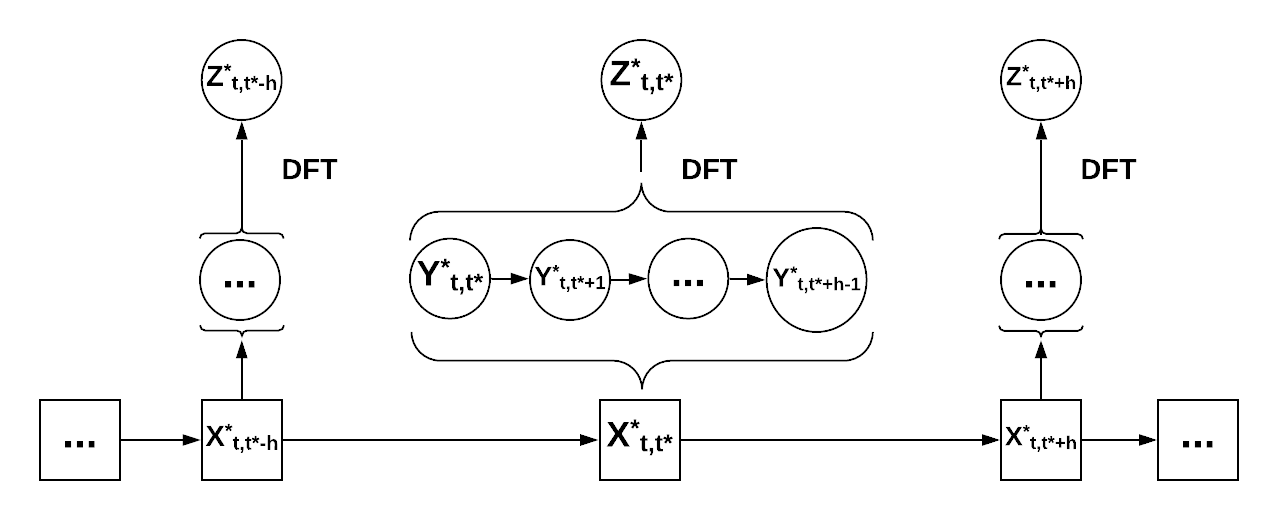
\includegraphics[width=4in]{../Plots/HMM-DFT.png}  
      \caption{HMM with Discrete Fourier Transform (\textbf{HMM-DFT})}
      \label{fig:HMM-DFT}
    \end{subfigure}
    \caption{Graphical representations of HMM models}
    \label{fig:models}
\end{figure}

%%% simulation study %%%

\begin{figure}[ht]
	\centering
	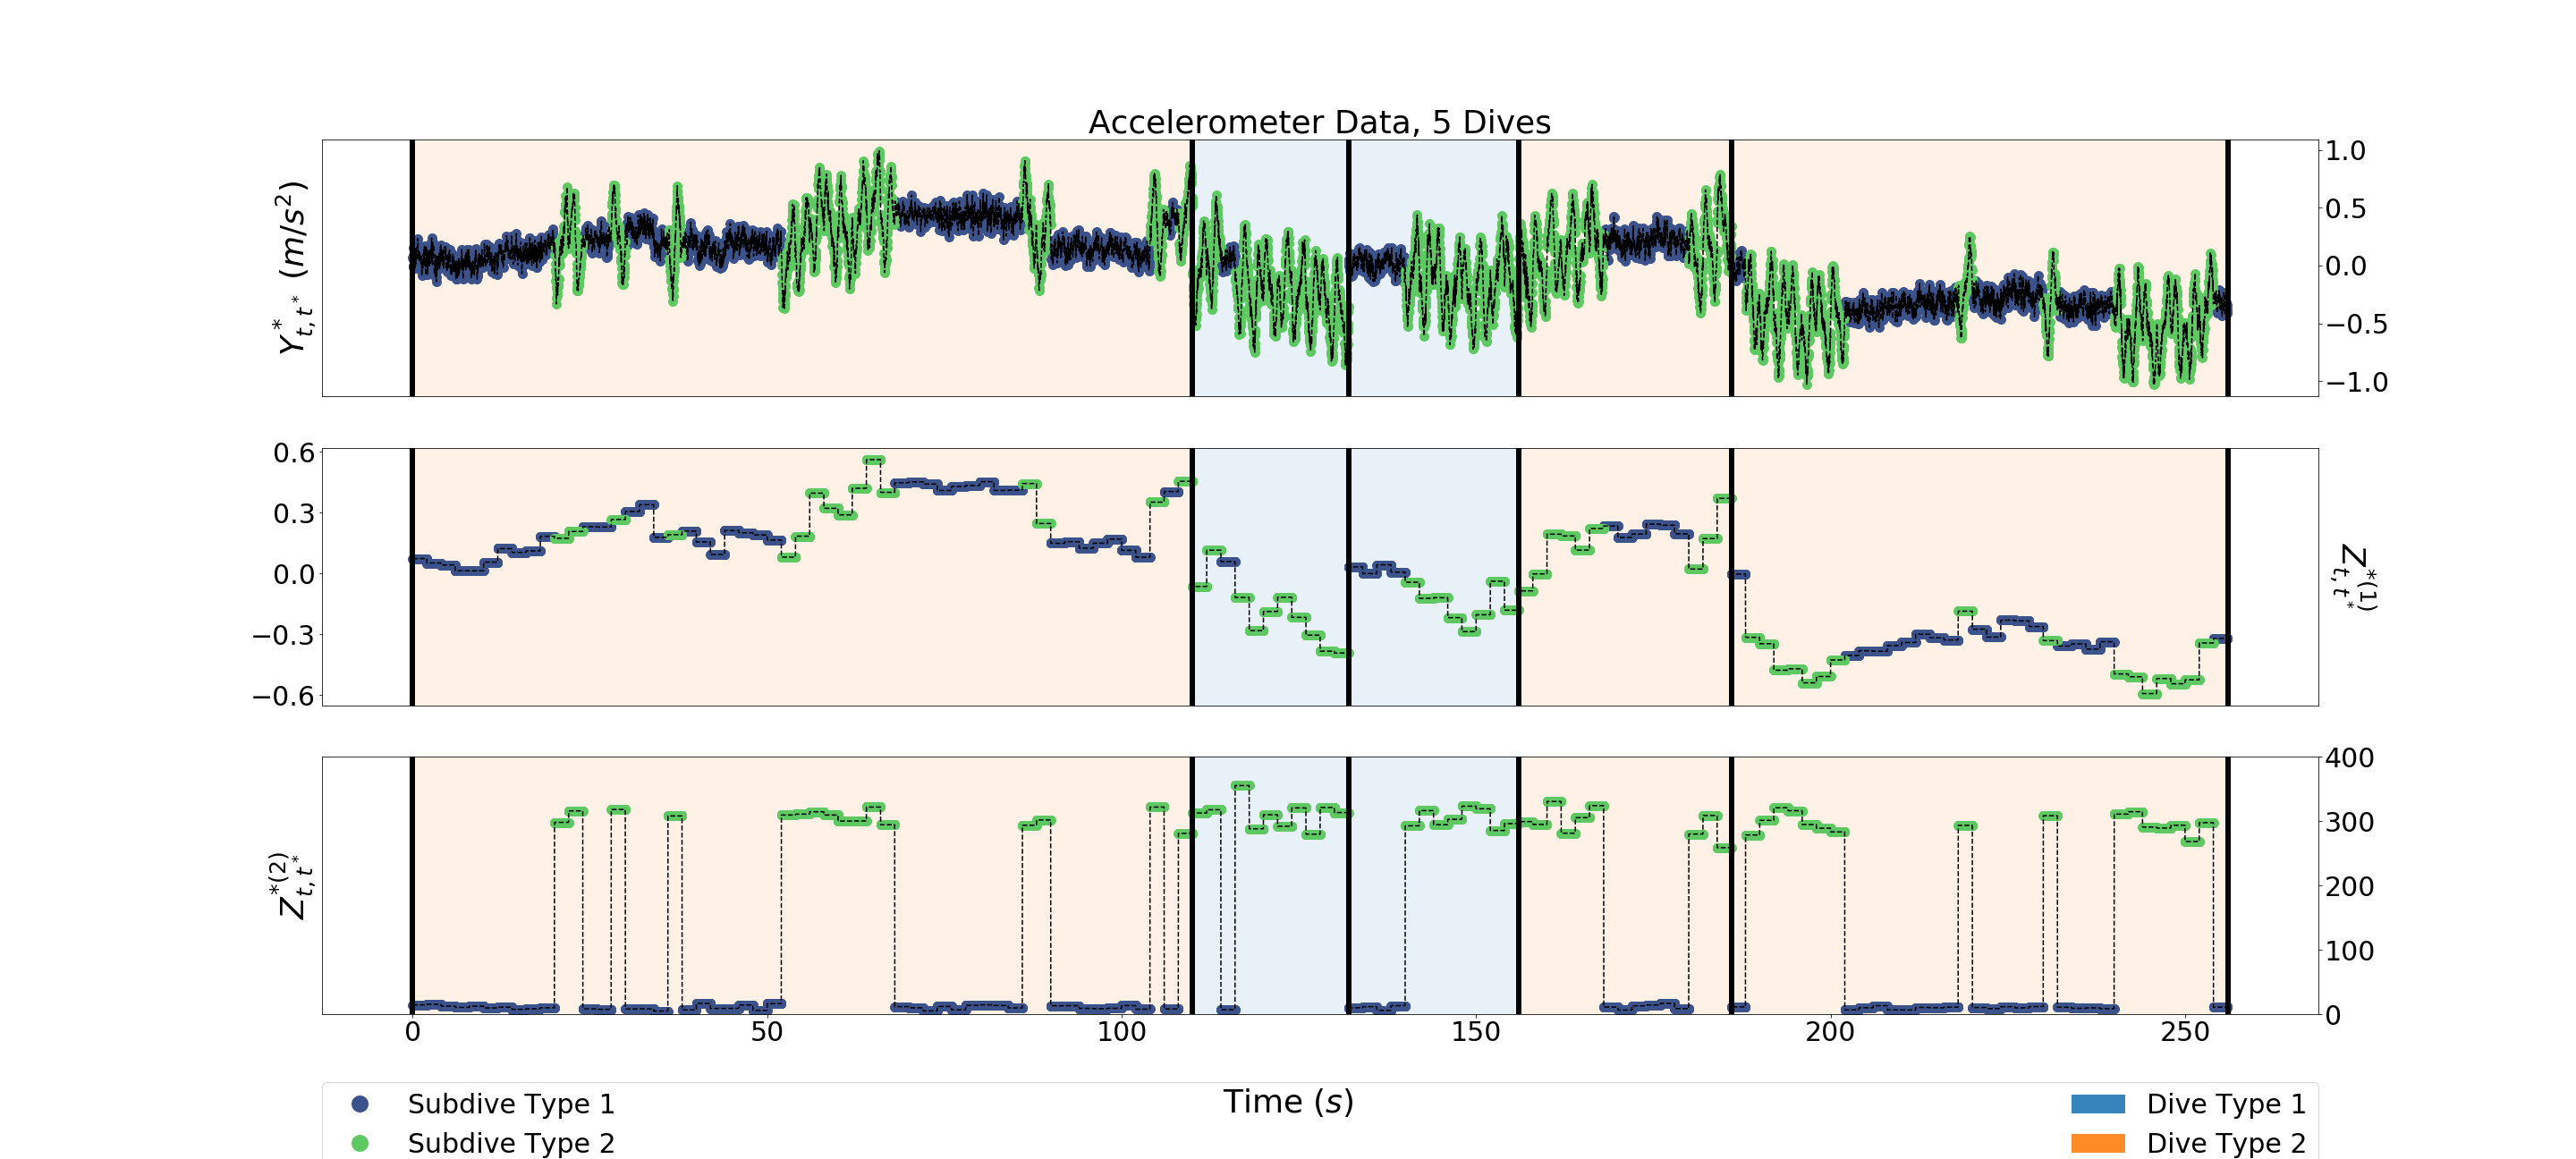
\includegraphics[width=5in]{../Plots/sim_data.png}
	\caption{Simulated acceleration data for one dive. The color of the line corresponds to the true fine-scale state of the subdive process, while the color of the background corresponds to the true dive type of the simulated whale.}
	\label{fig:sim_data}
\end{figure}

\begin{figure}[ht]
	\centering
	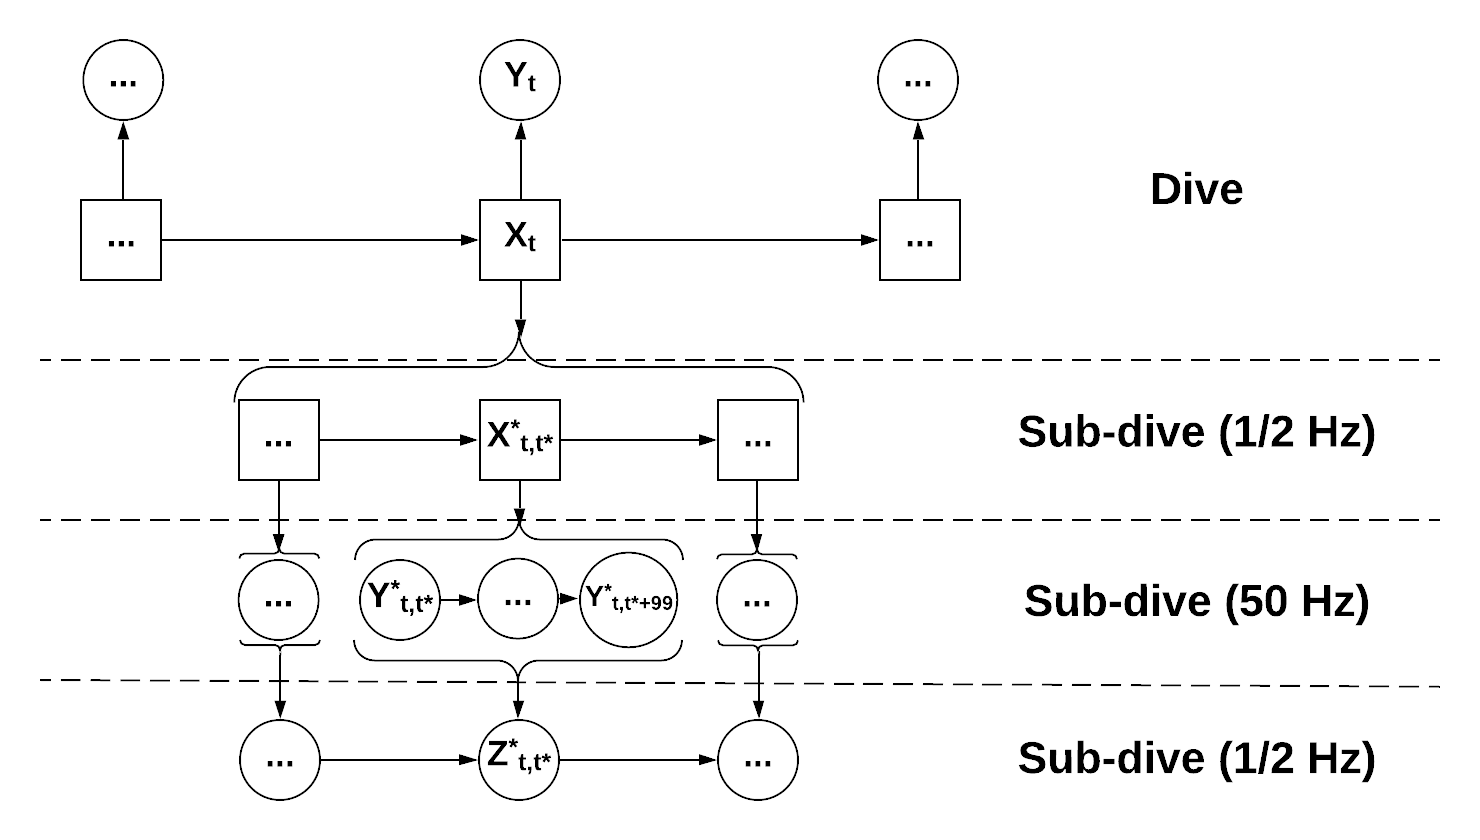
\includegraphics[width=5in]{../Plots/CarHHMM-DFT.png}
	\caption{Graphical representation the model used in the simulation and case study, the \textbf{CarHHMM-DFT}.}
	\label{fig:CarHHMM-DFT}
\end{figure}

\begin{figure}[ht]
    \centering
    \begin{subfigure}[t]{1.0\textwidth}
        \centering
        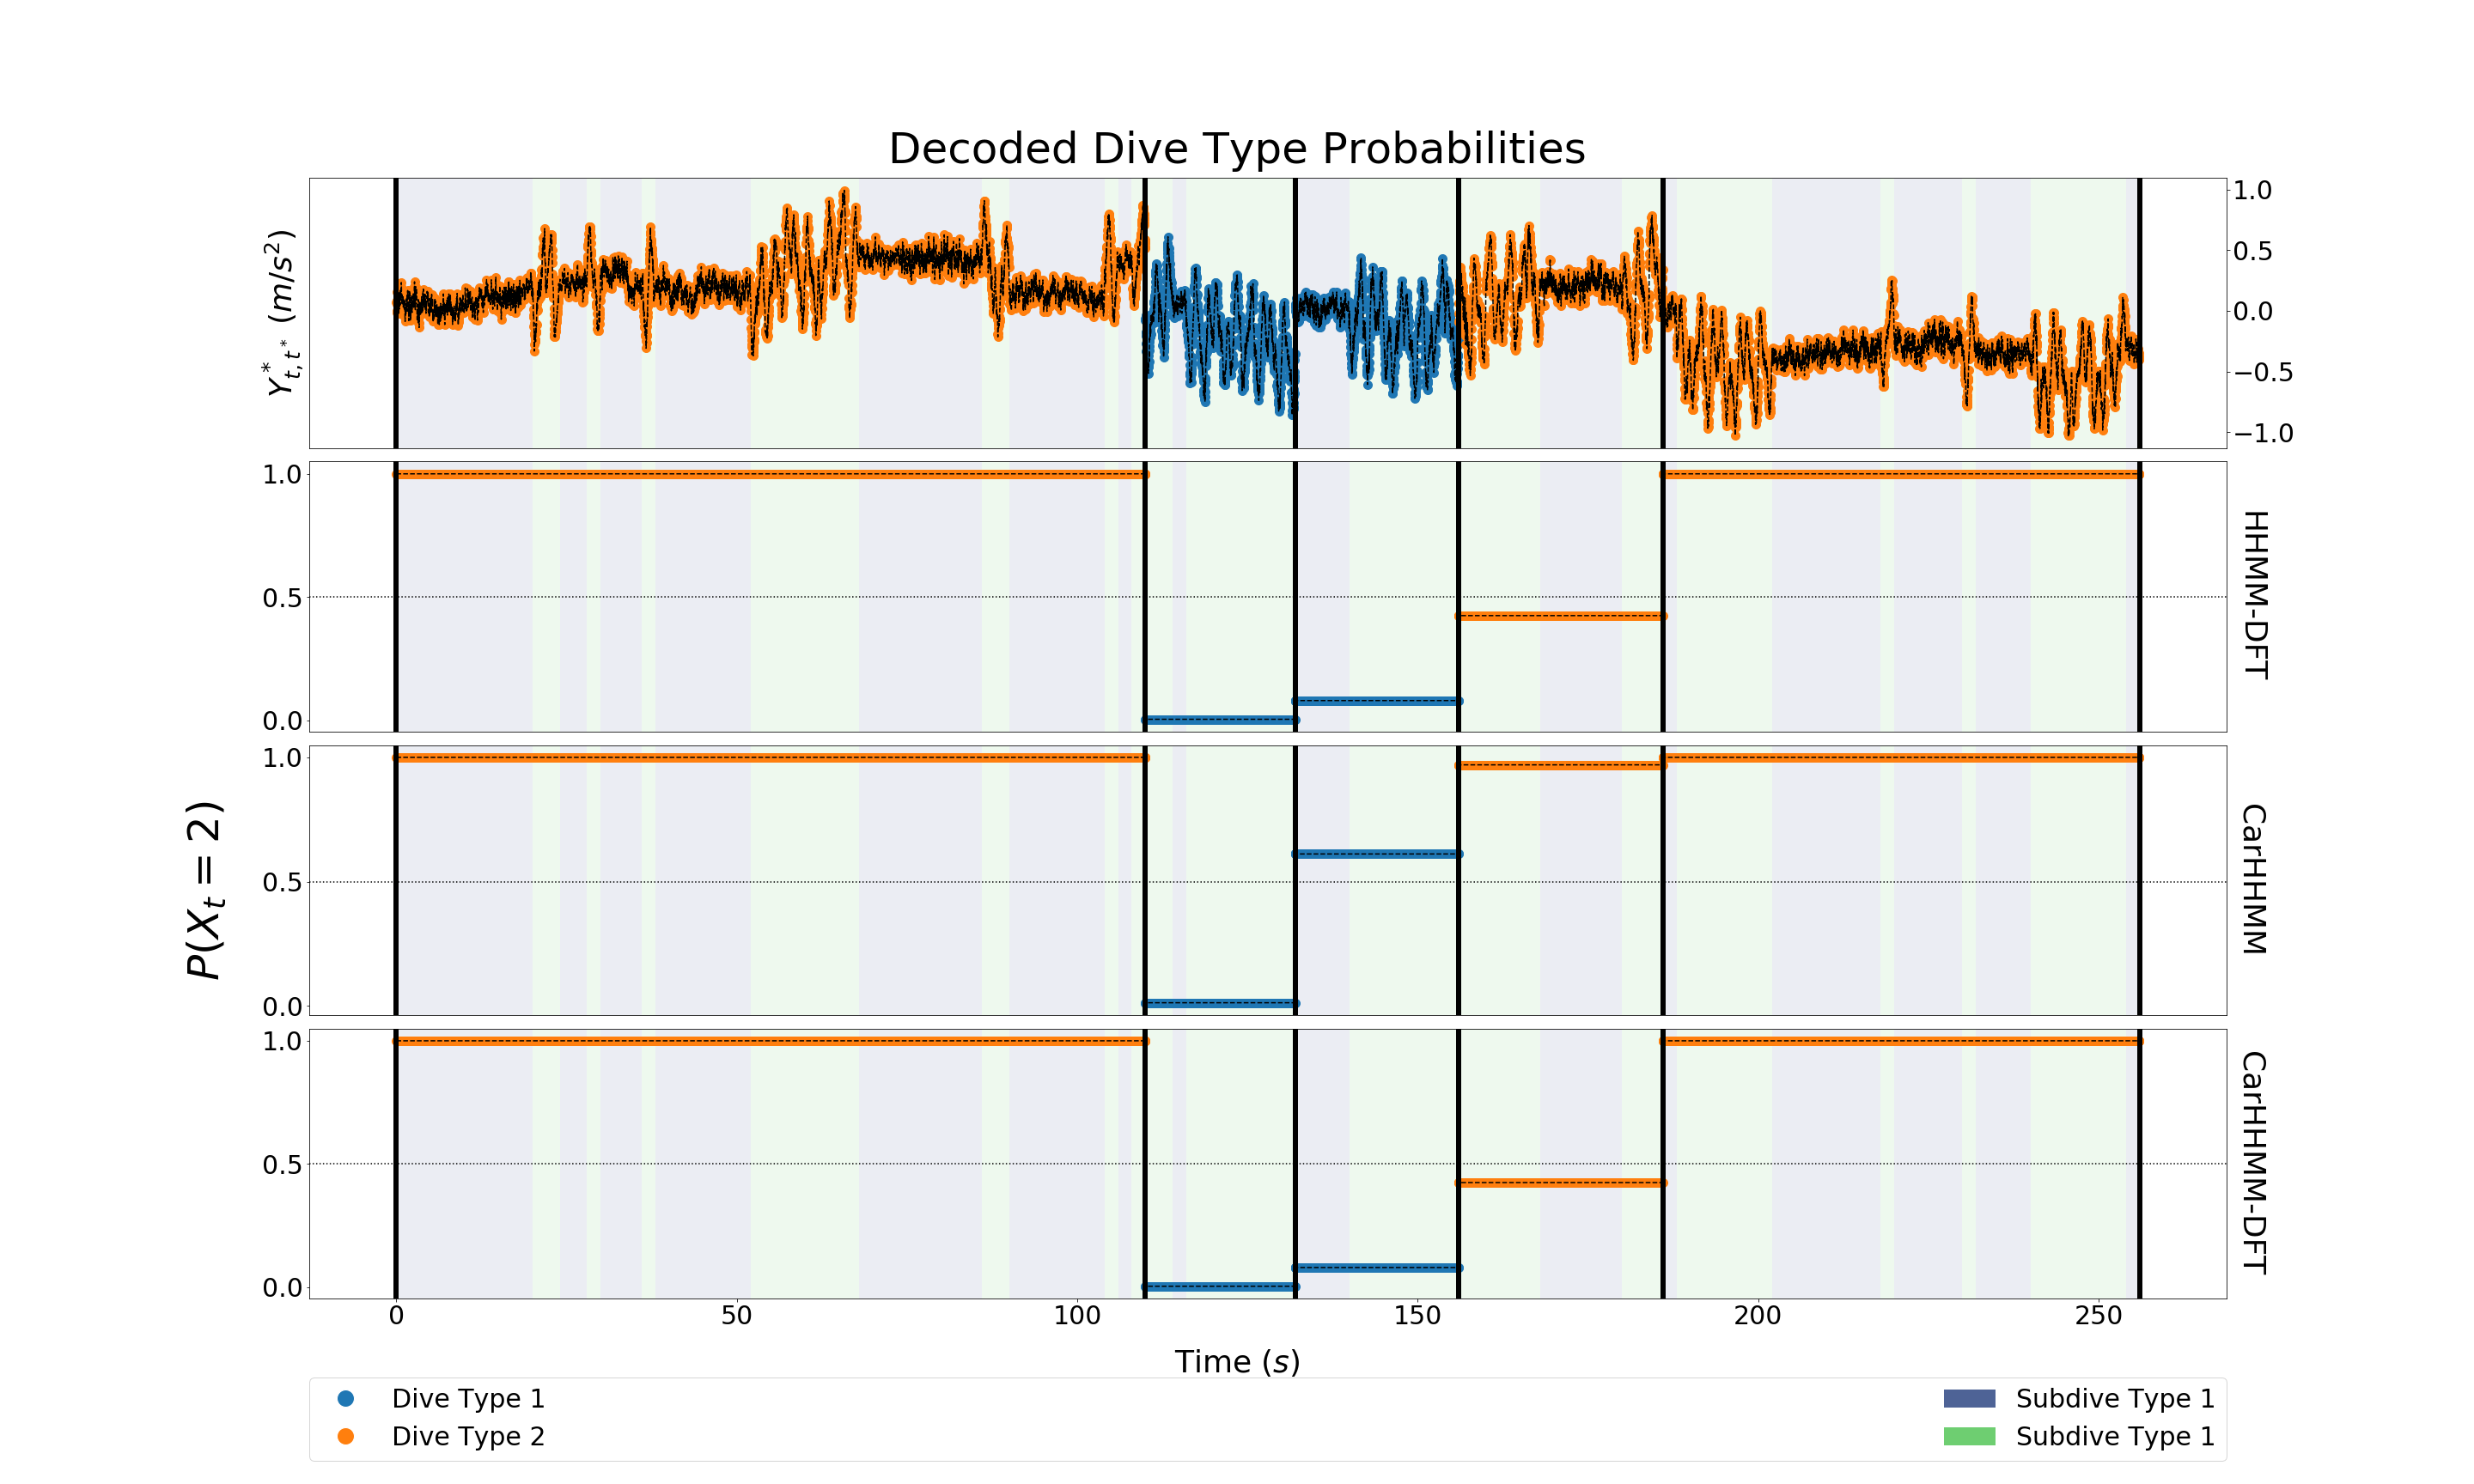
\includegraphics[width=3.5in]{../Plots/Posterior_Coarse_States.png}
        \caption{Coarse-scale hidden process}
    \end{subfigure}
    %
    \begin{subfigure}[t]{1.0\textwidth}
        \centering
        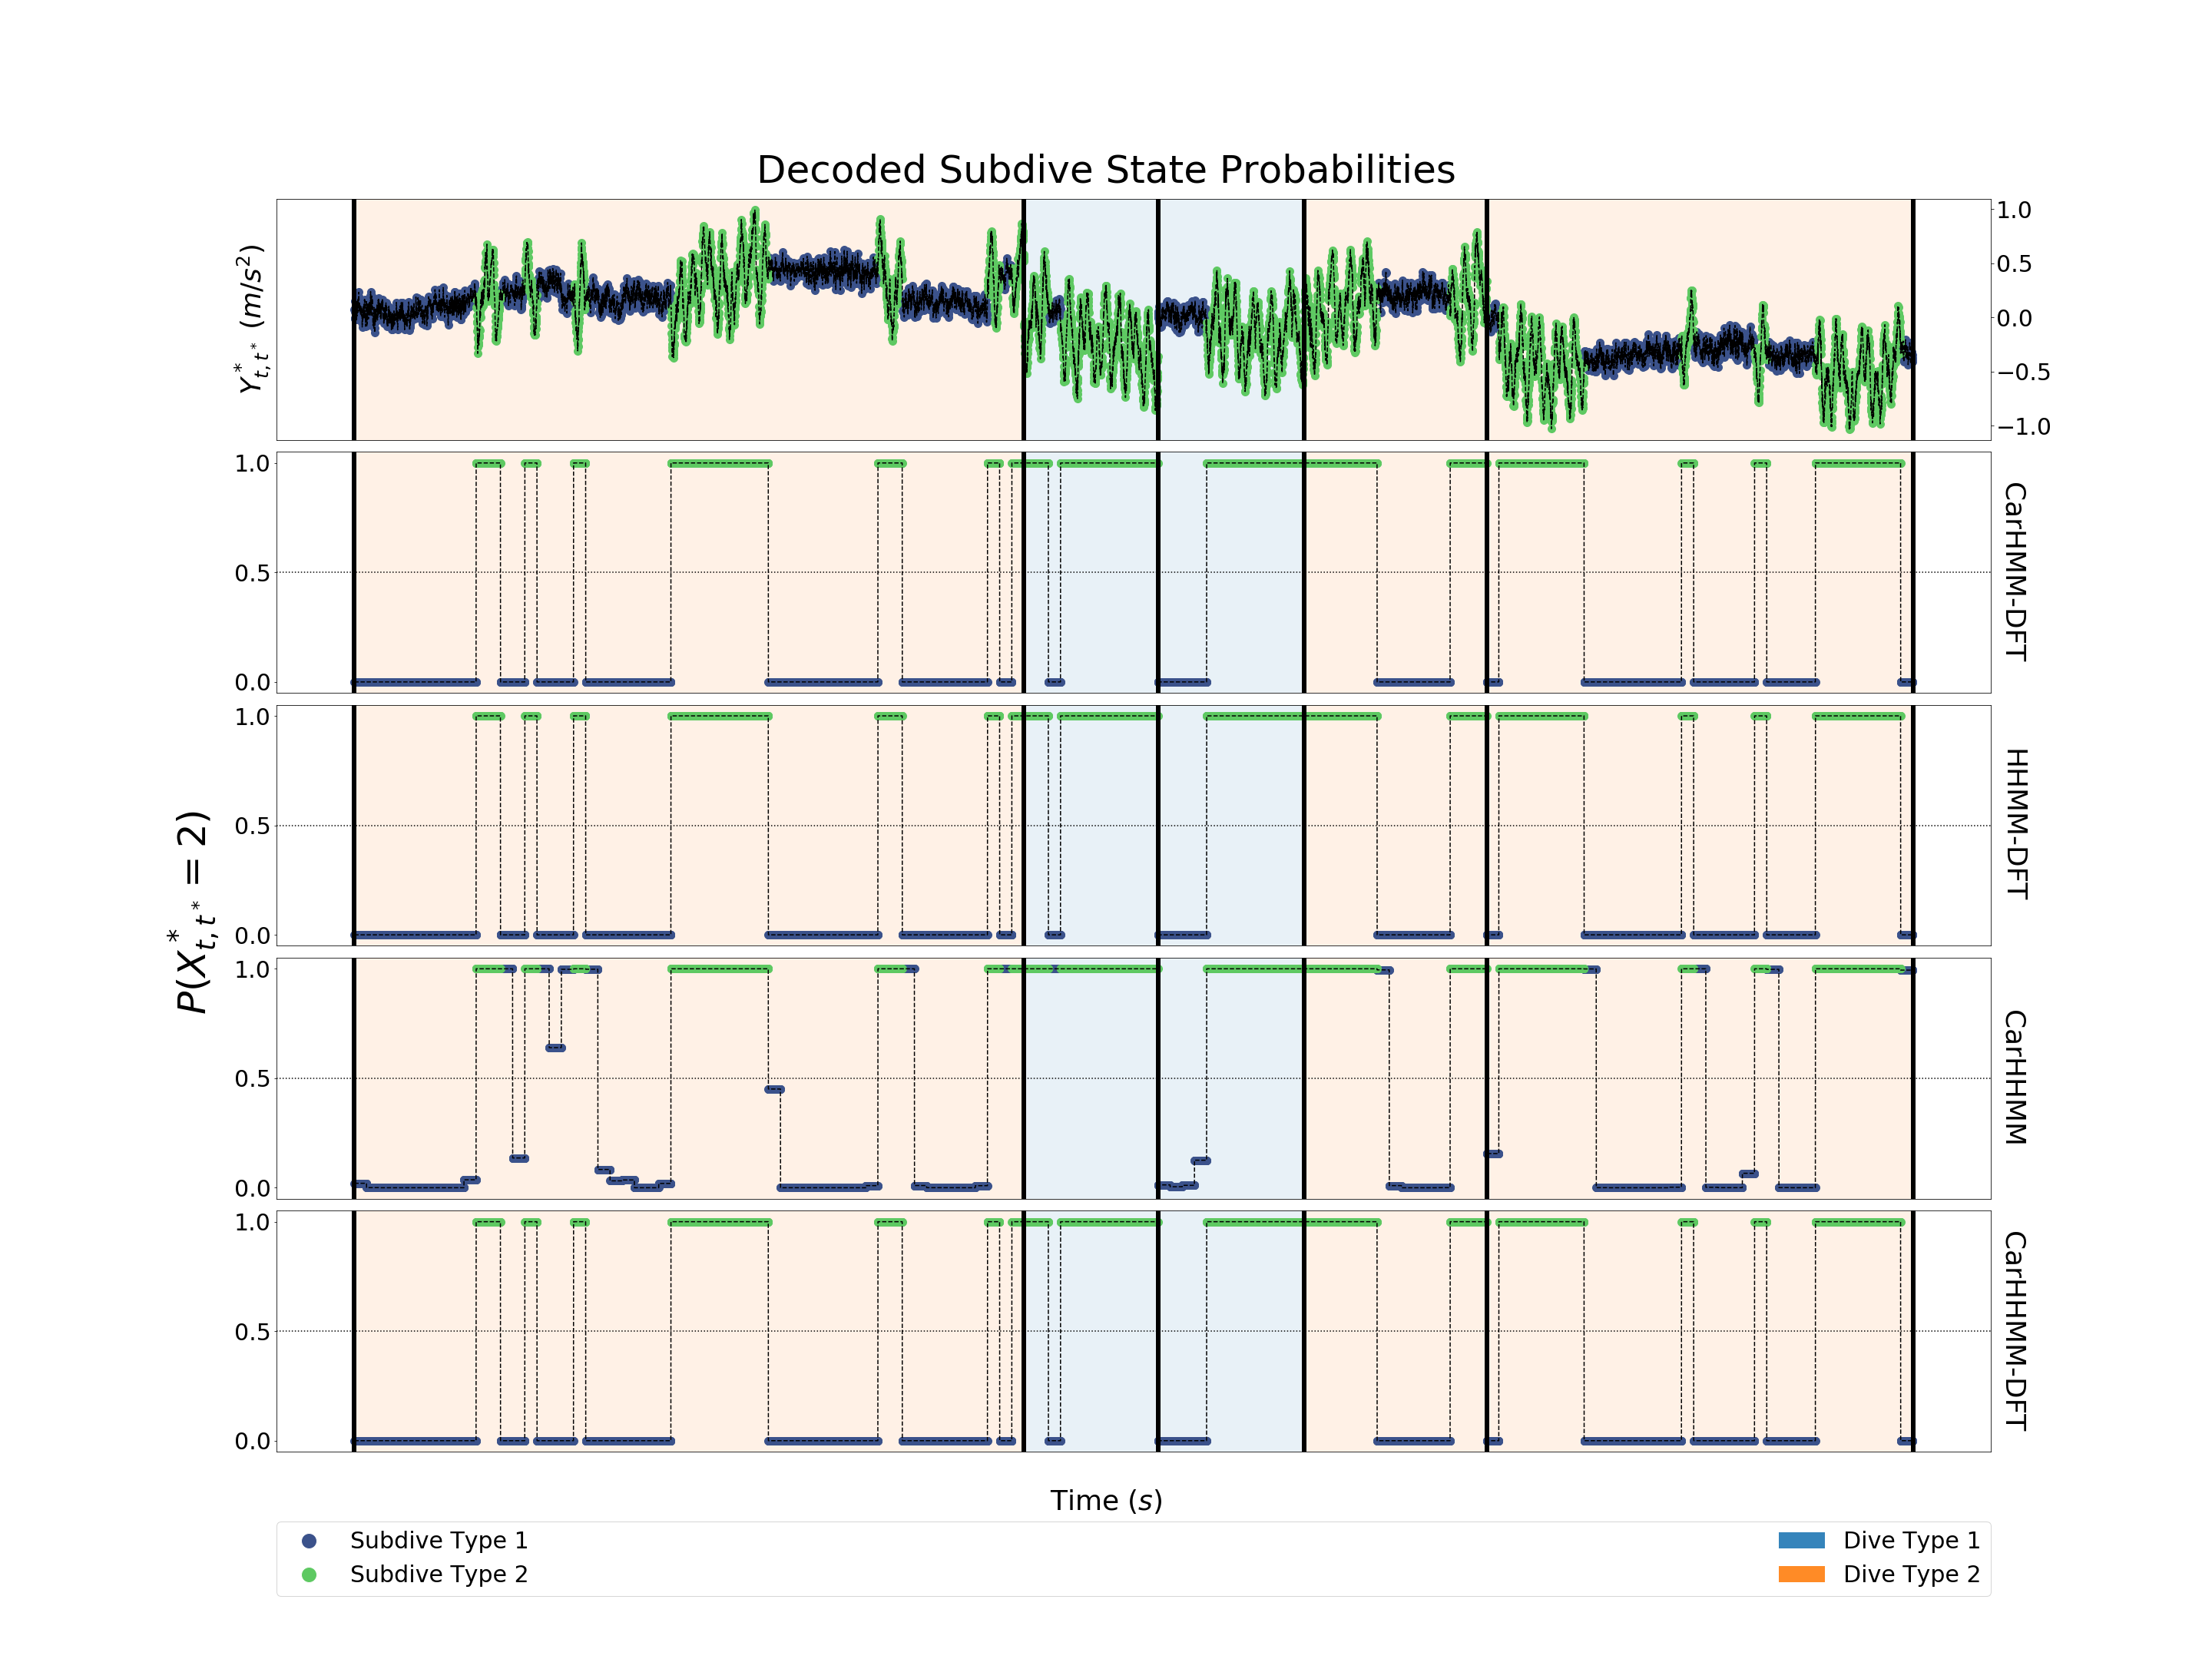
\includegraphics[width=3.5in]{../Plots/Posterior_Fine_States.png}
        \caption{Fine-scale hidden process}
    \end{subfigure}
	\caption{Decoded state probabilities of each model for 5 dives of one simulated data set. The colors correspond to the true behavioral state / dive type.}
	\label{fig:acc}
\end{figure}

%%% Case Study %%%

\begin{figure}[ht]
	\centering
	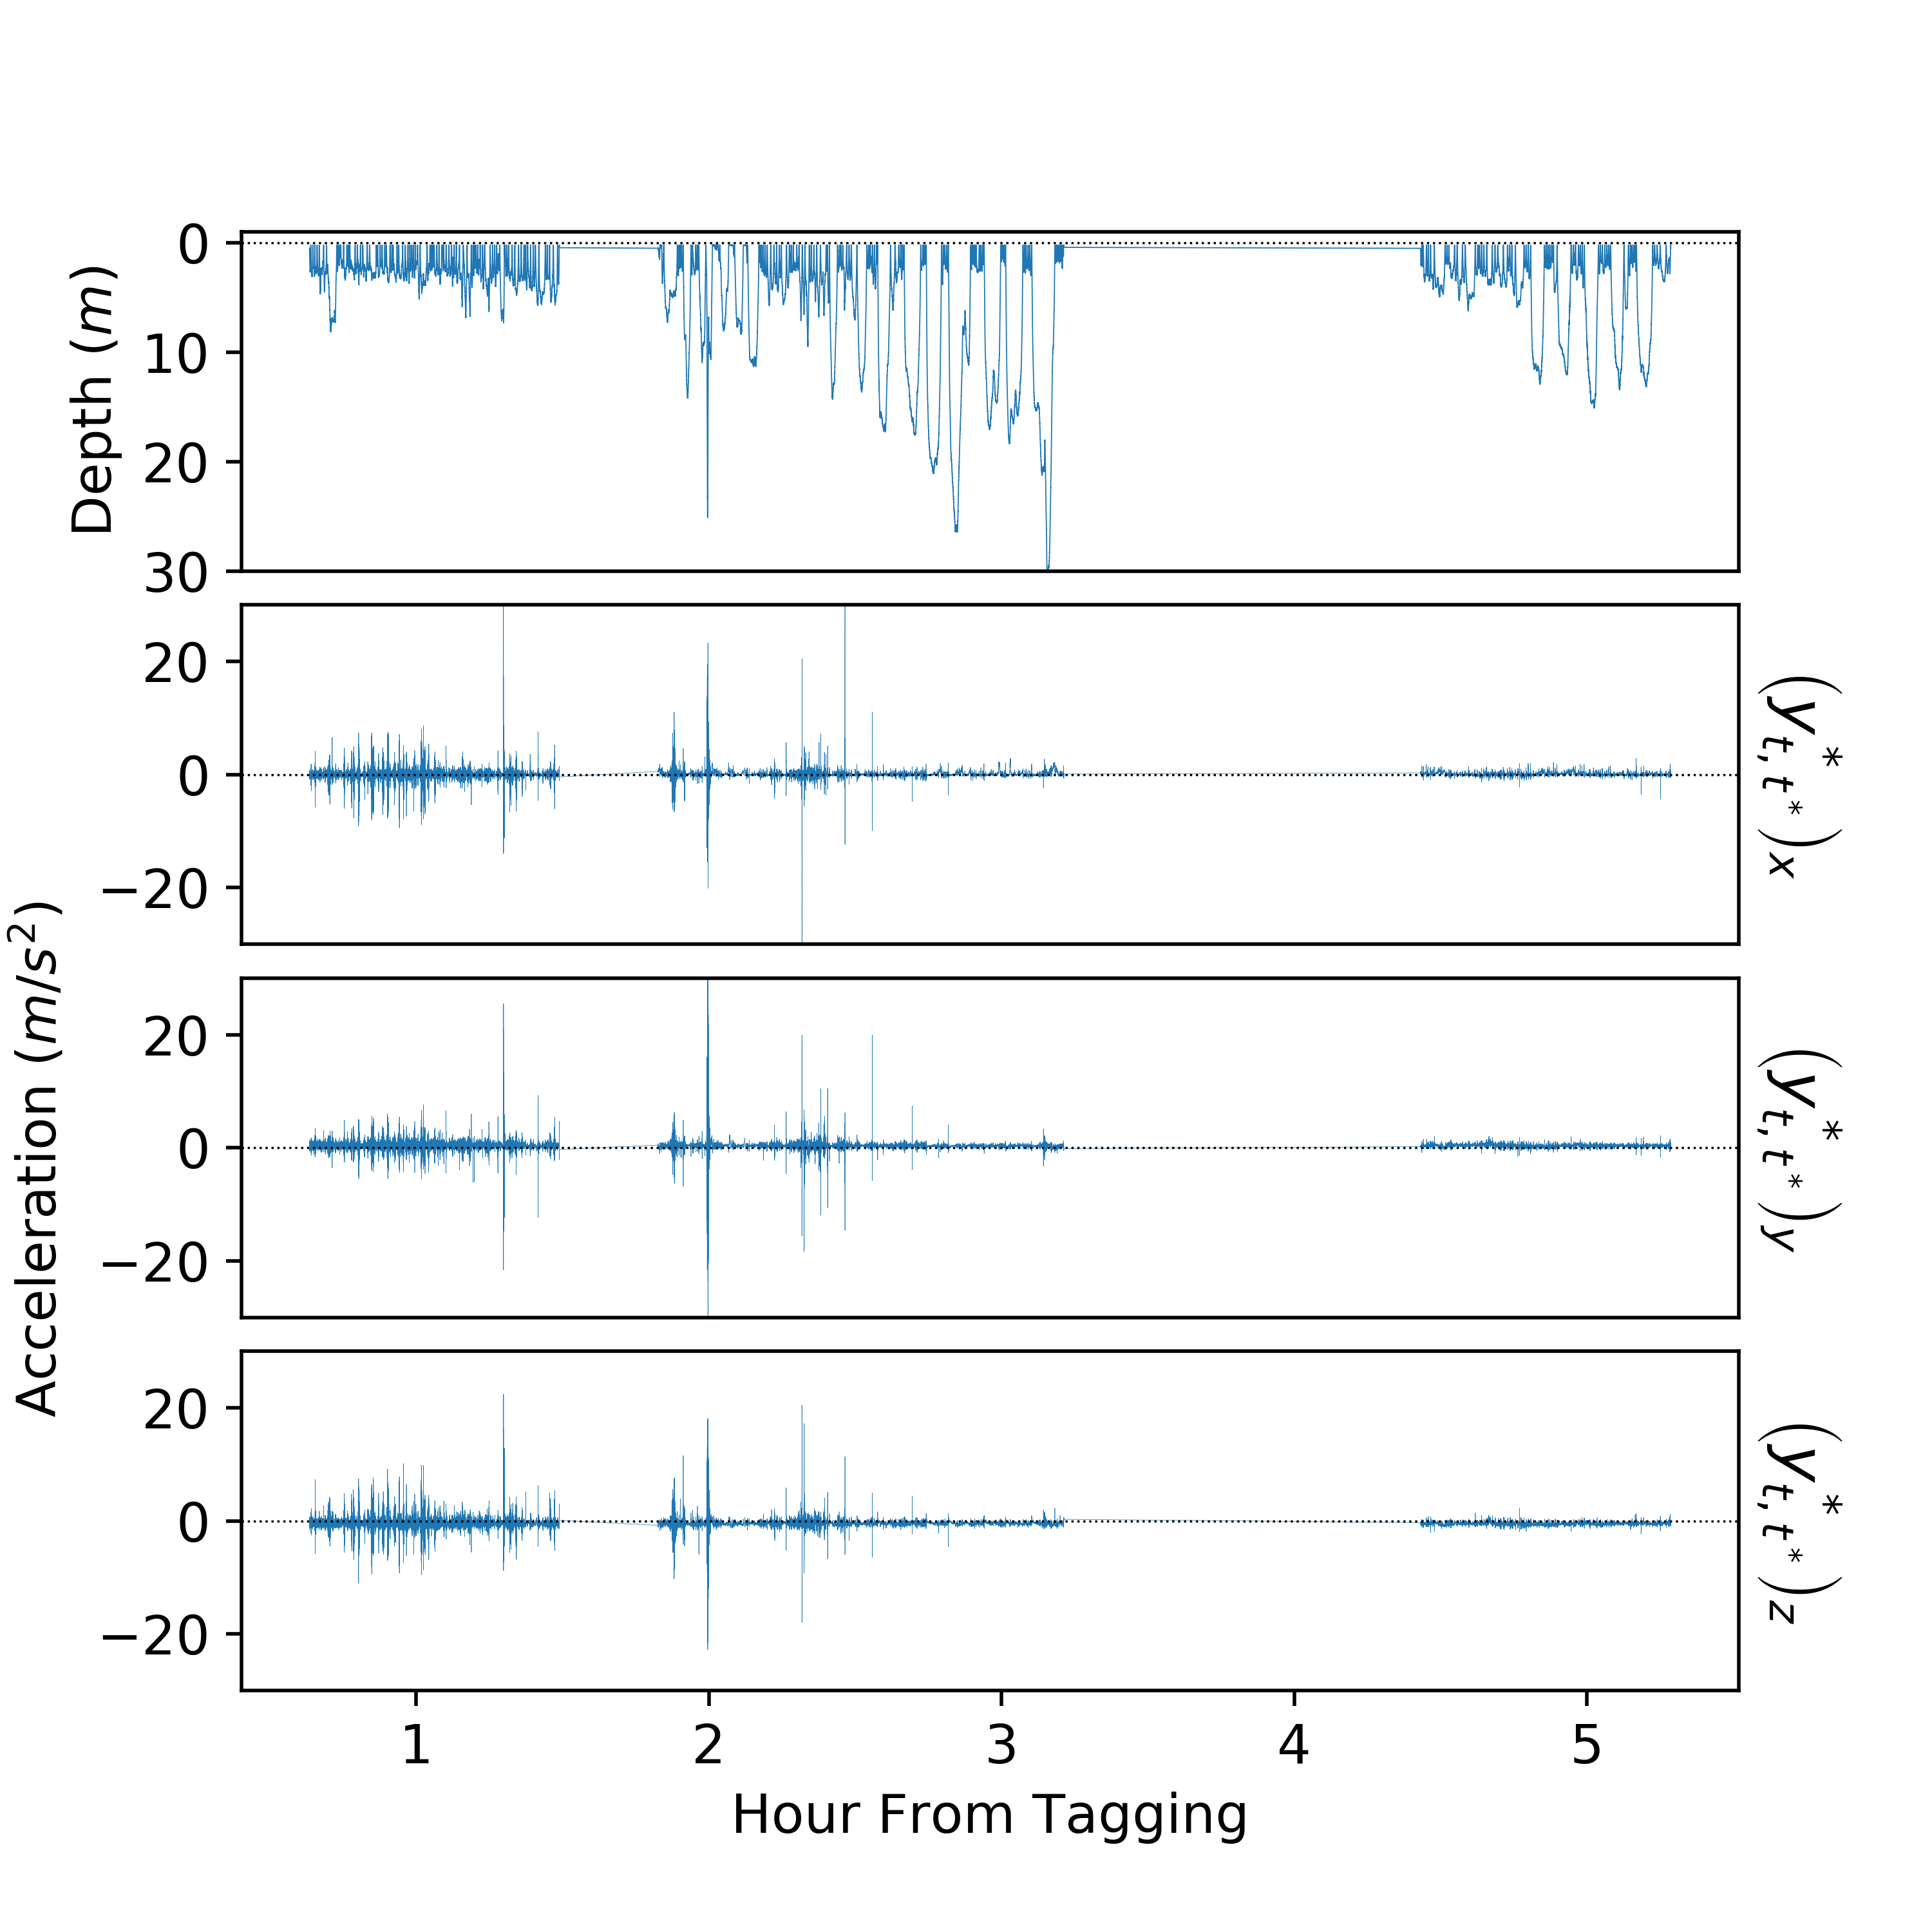
\includegraphics[width=5in]{../Plots/raw_data.png}
	\caption{Dive depth (top panel) and acceleration (bottom three panels) as functions of time, from the killer whale data set}
	\label{fig:data}
\end{figure}

\begin{figure}[ht]
	\centering
	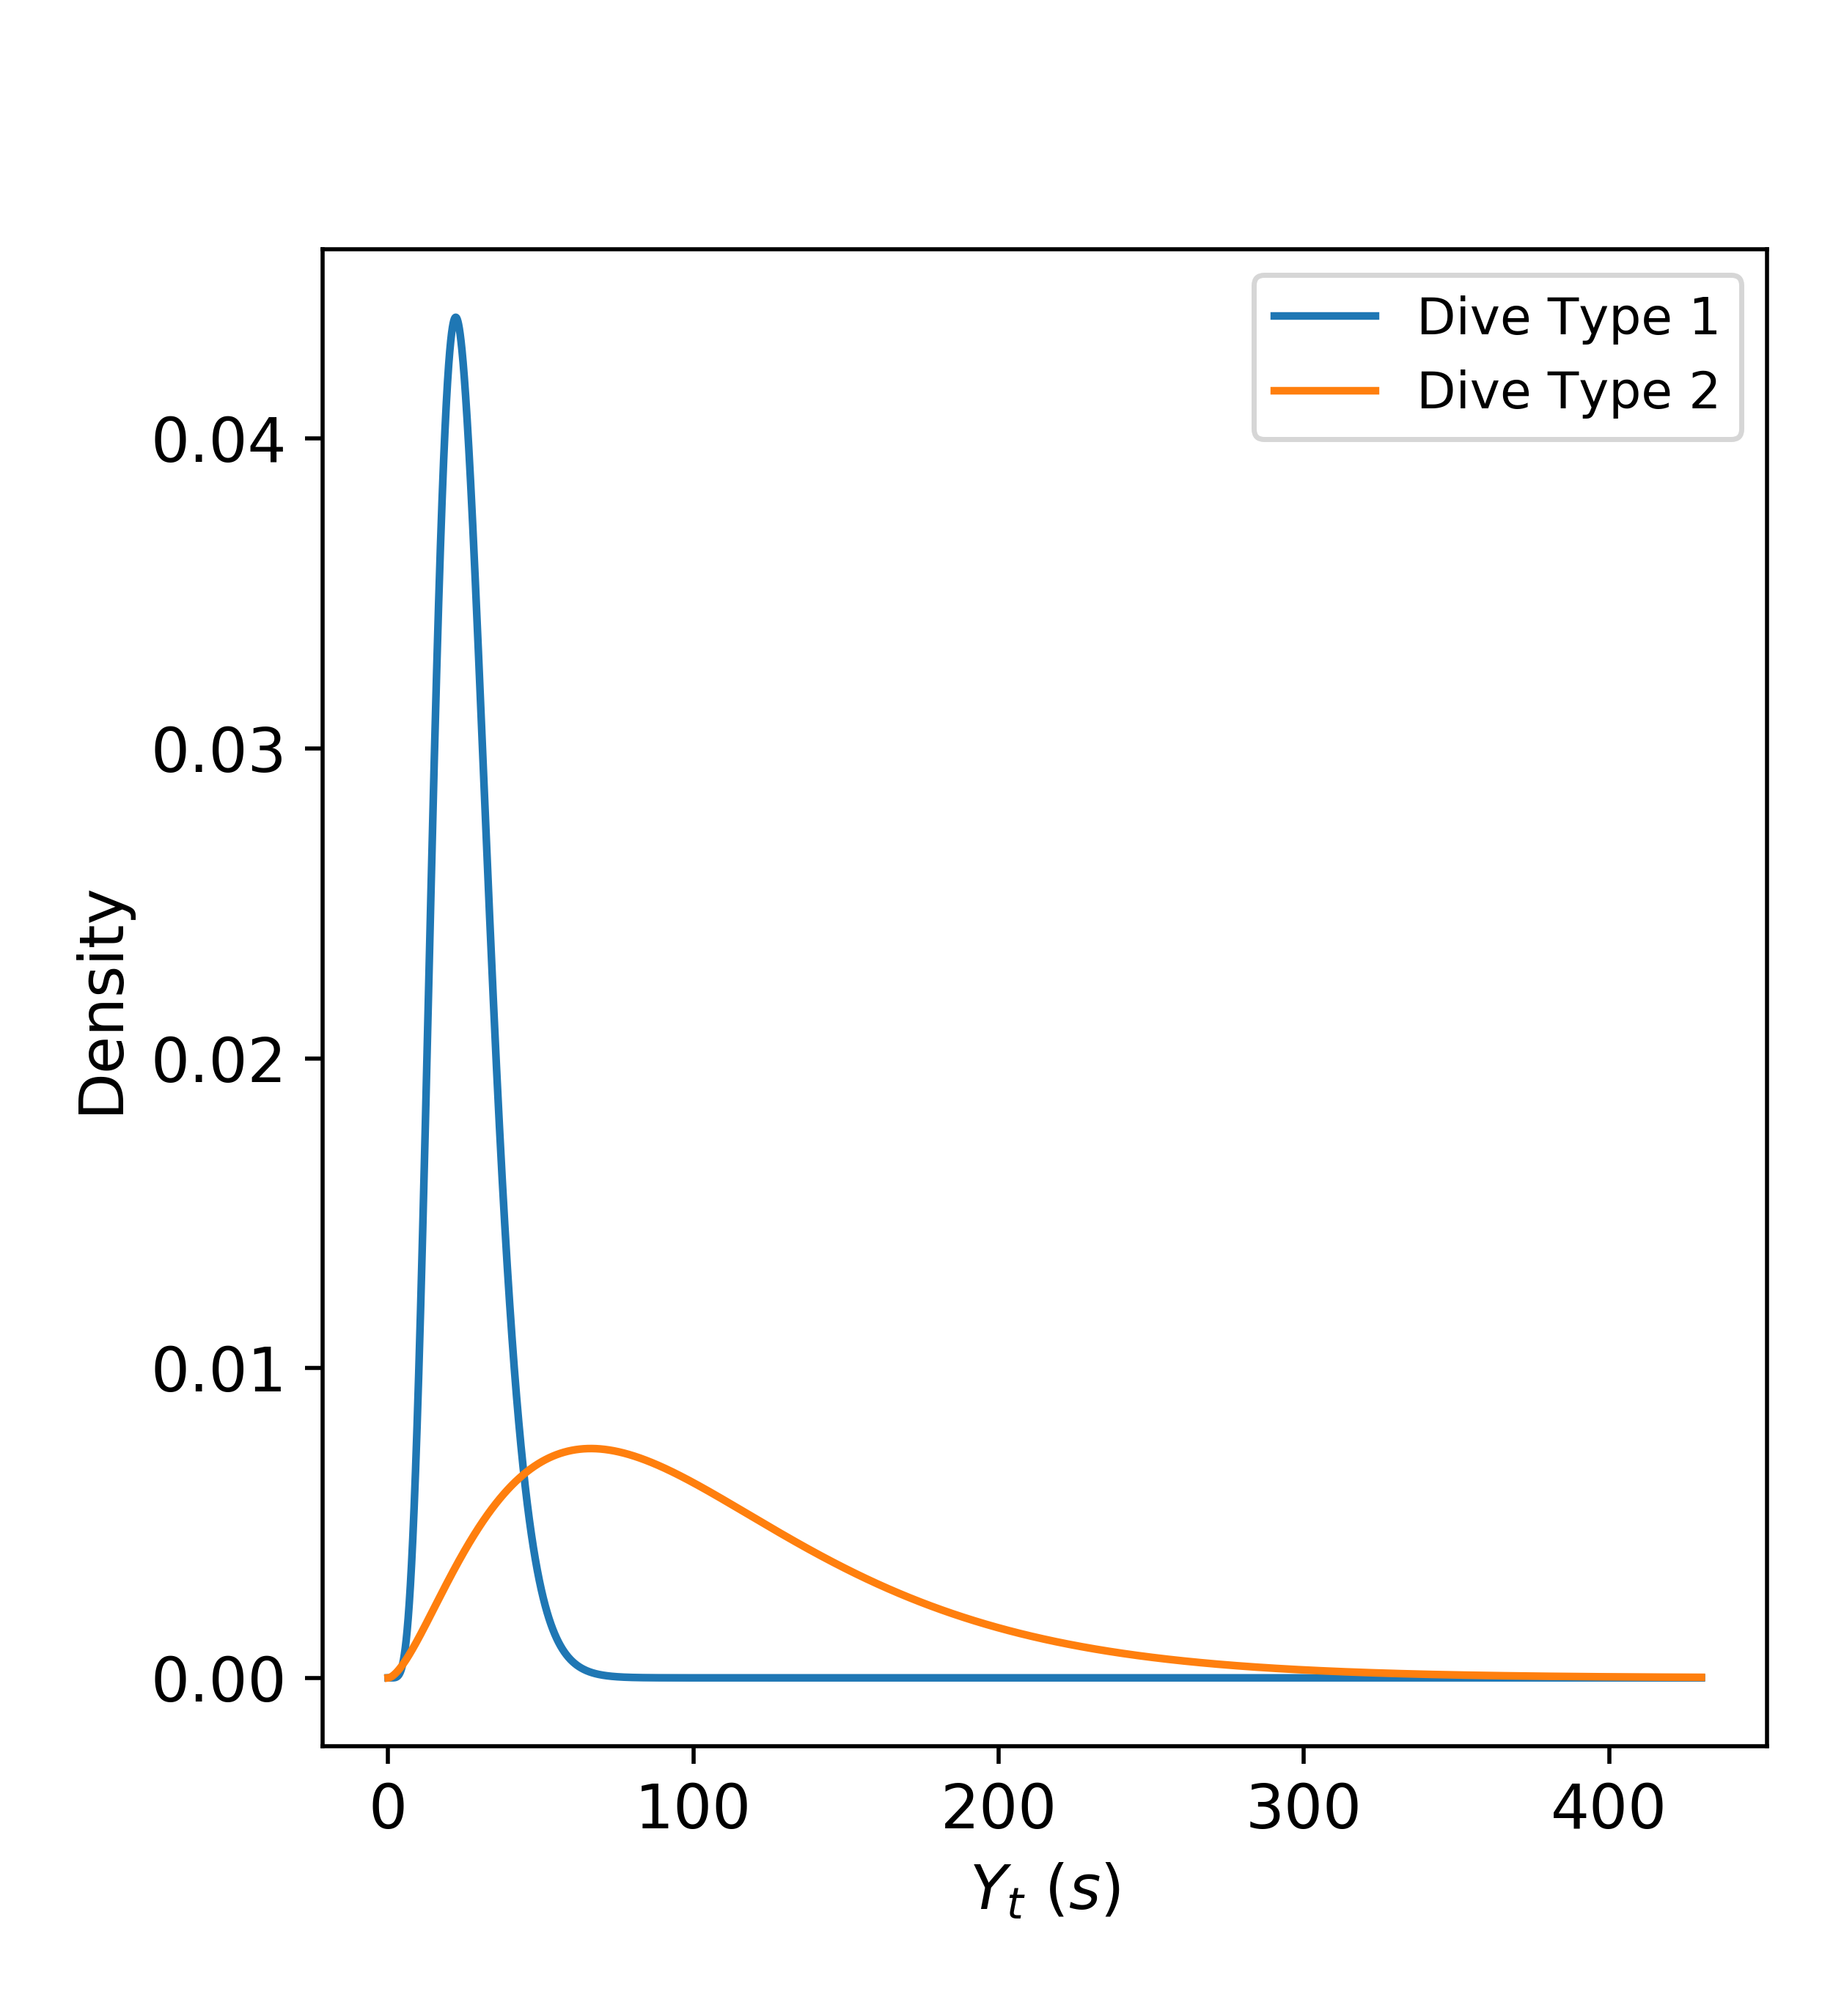
\includegraphics[width=5in]{../Plots/CarHHMM2-coarse-emissions.png}
	\caption{Estimated probability distributions for each coarse-scale observation in each dive type.}
	\label{fig:coarse_emis}
\end{figure}

\begin{figure}[ht]
	\centering
	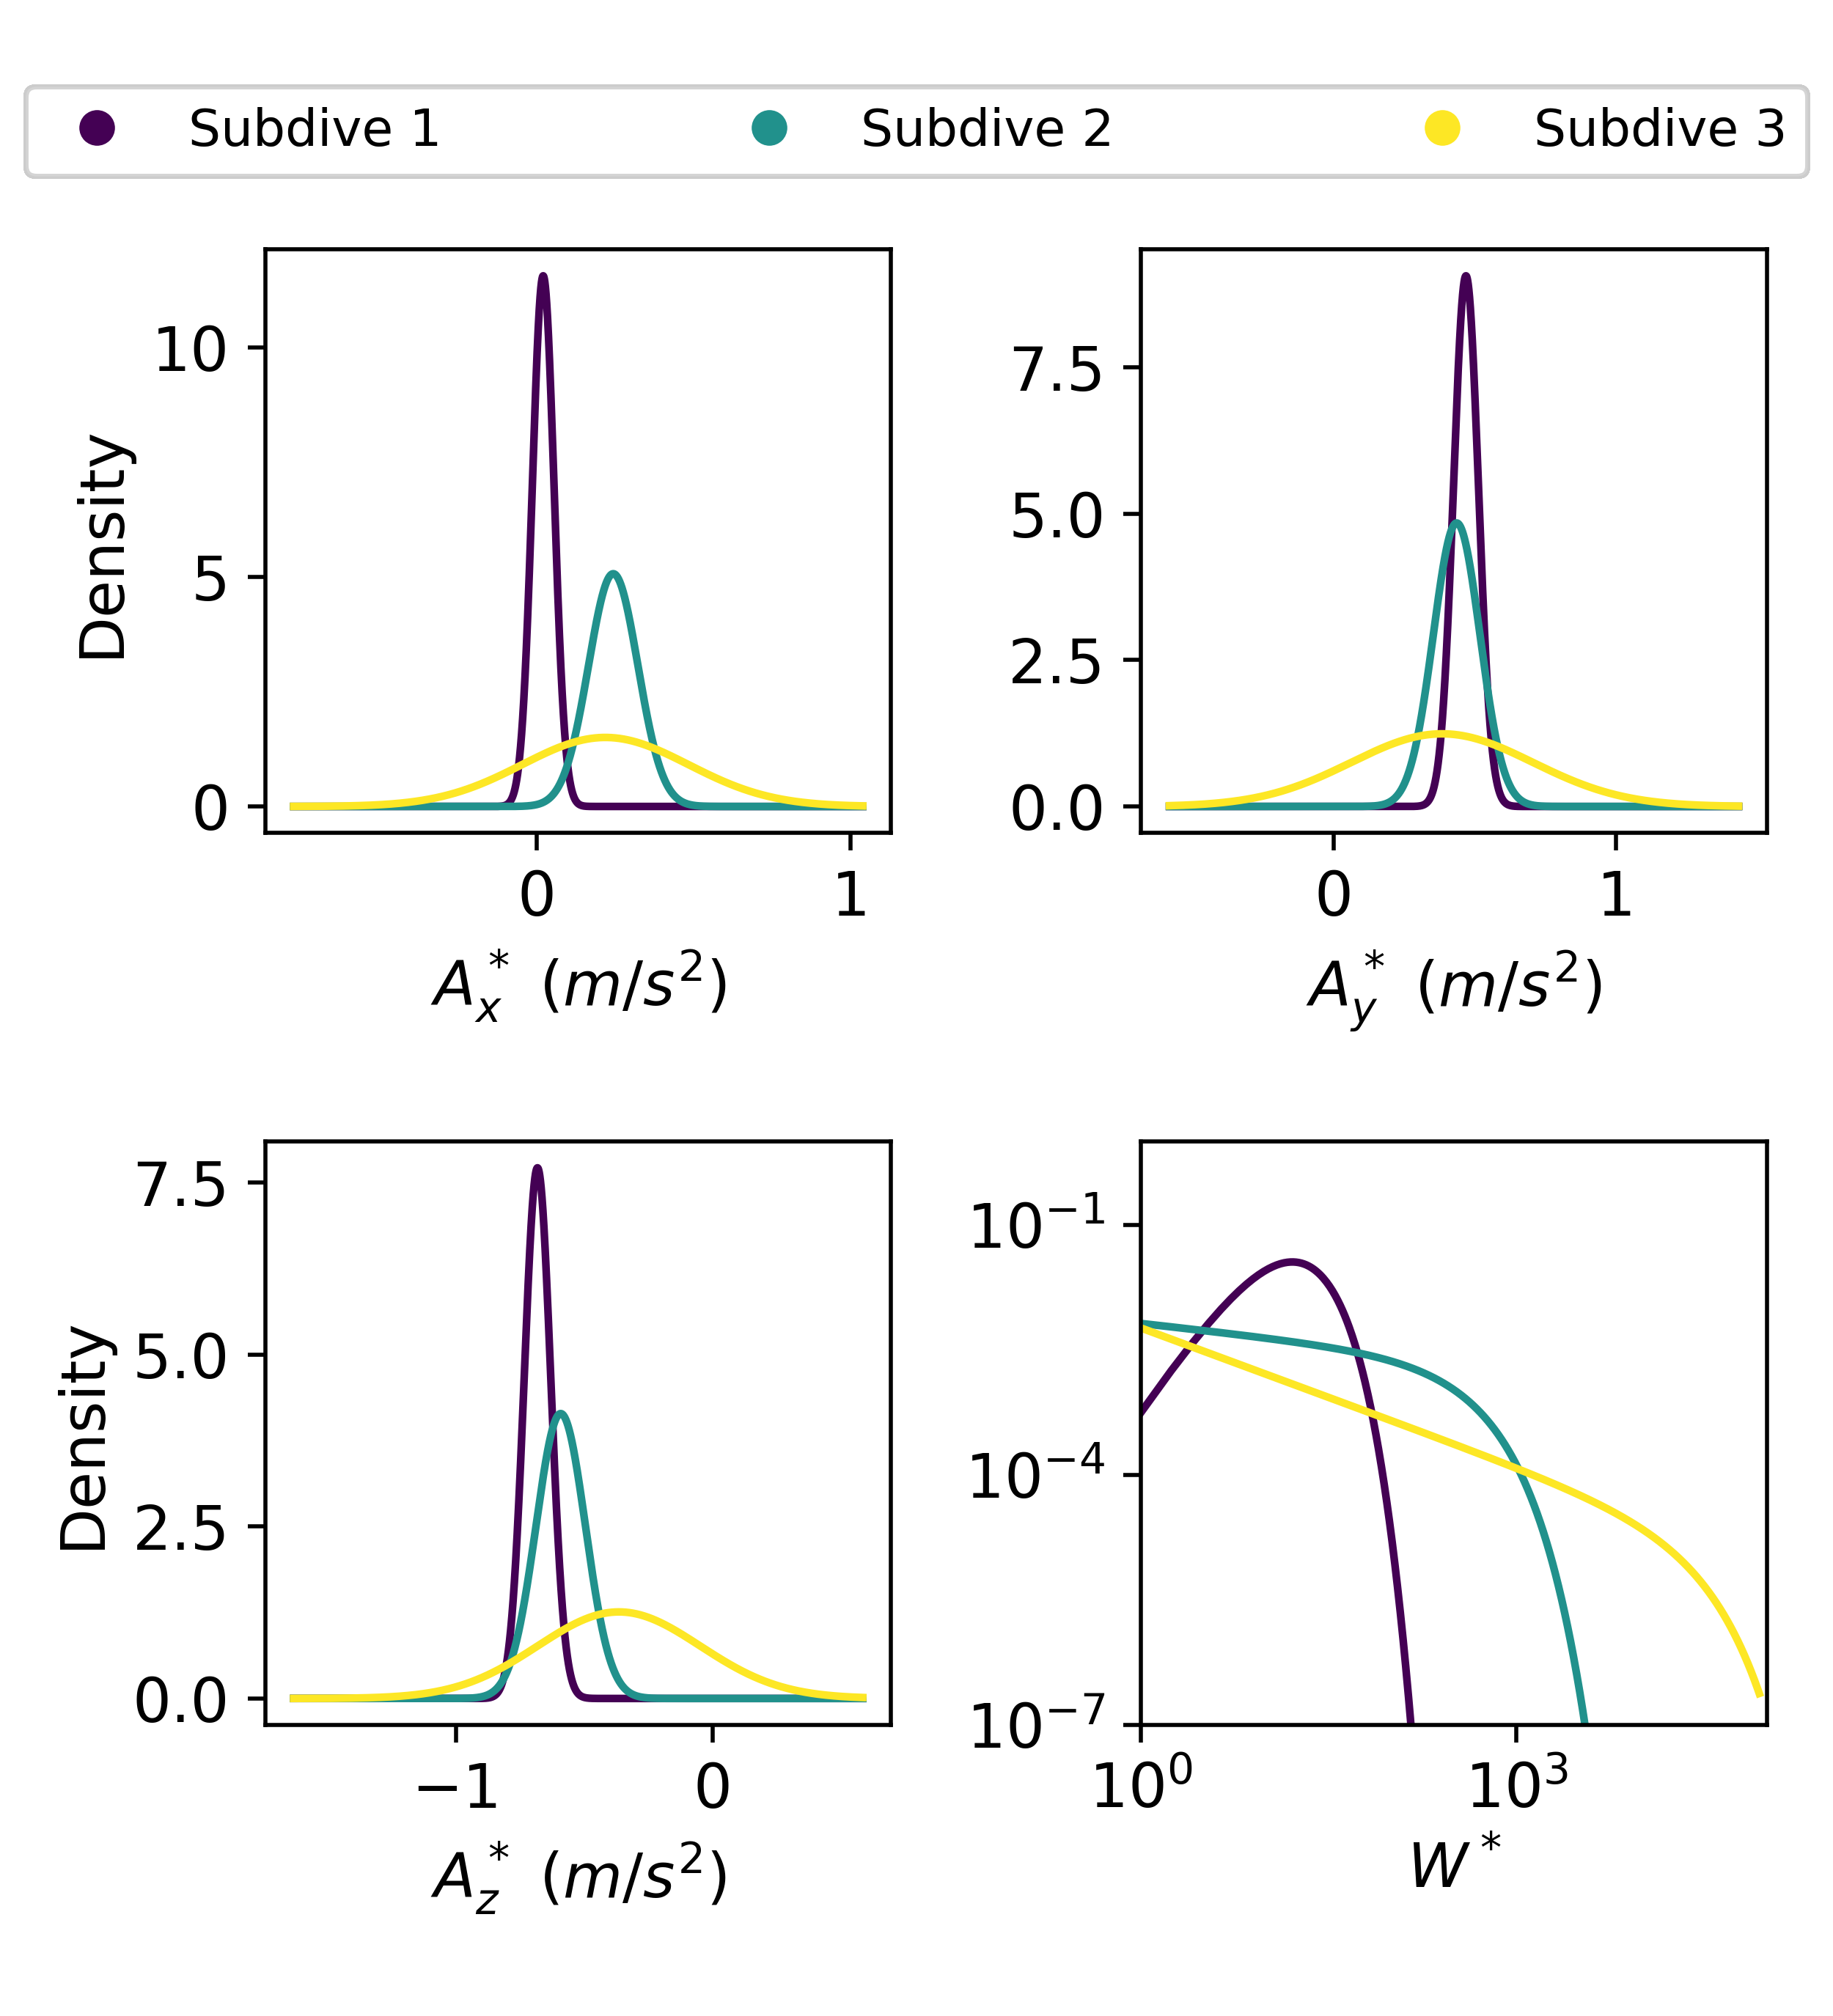
\includegraphics[width=5in]{../Plots/CarHHMM2-fine-emissions.png}
	\caption{Estimated probability distributions for each fine-scale observation in each behavioral state. Note that the distributions of acceleration do not take auto-correlation into account (see Table \ref{table:emis_dists_CarHHMM-DFT})}
	\label{fig:fine_emis}
\end{figure}

\begin{figure}[ht]
	\centering
	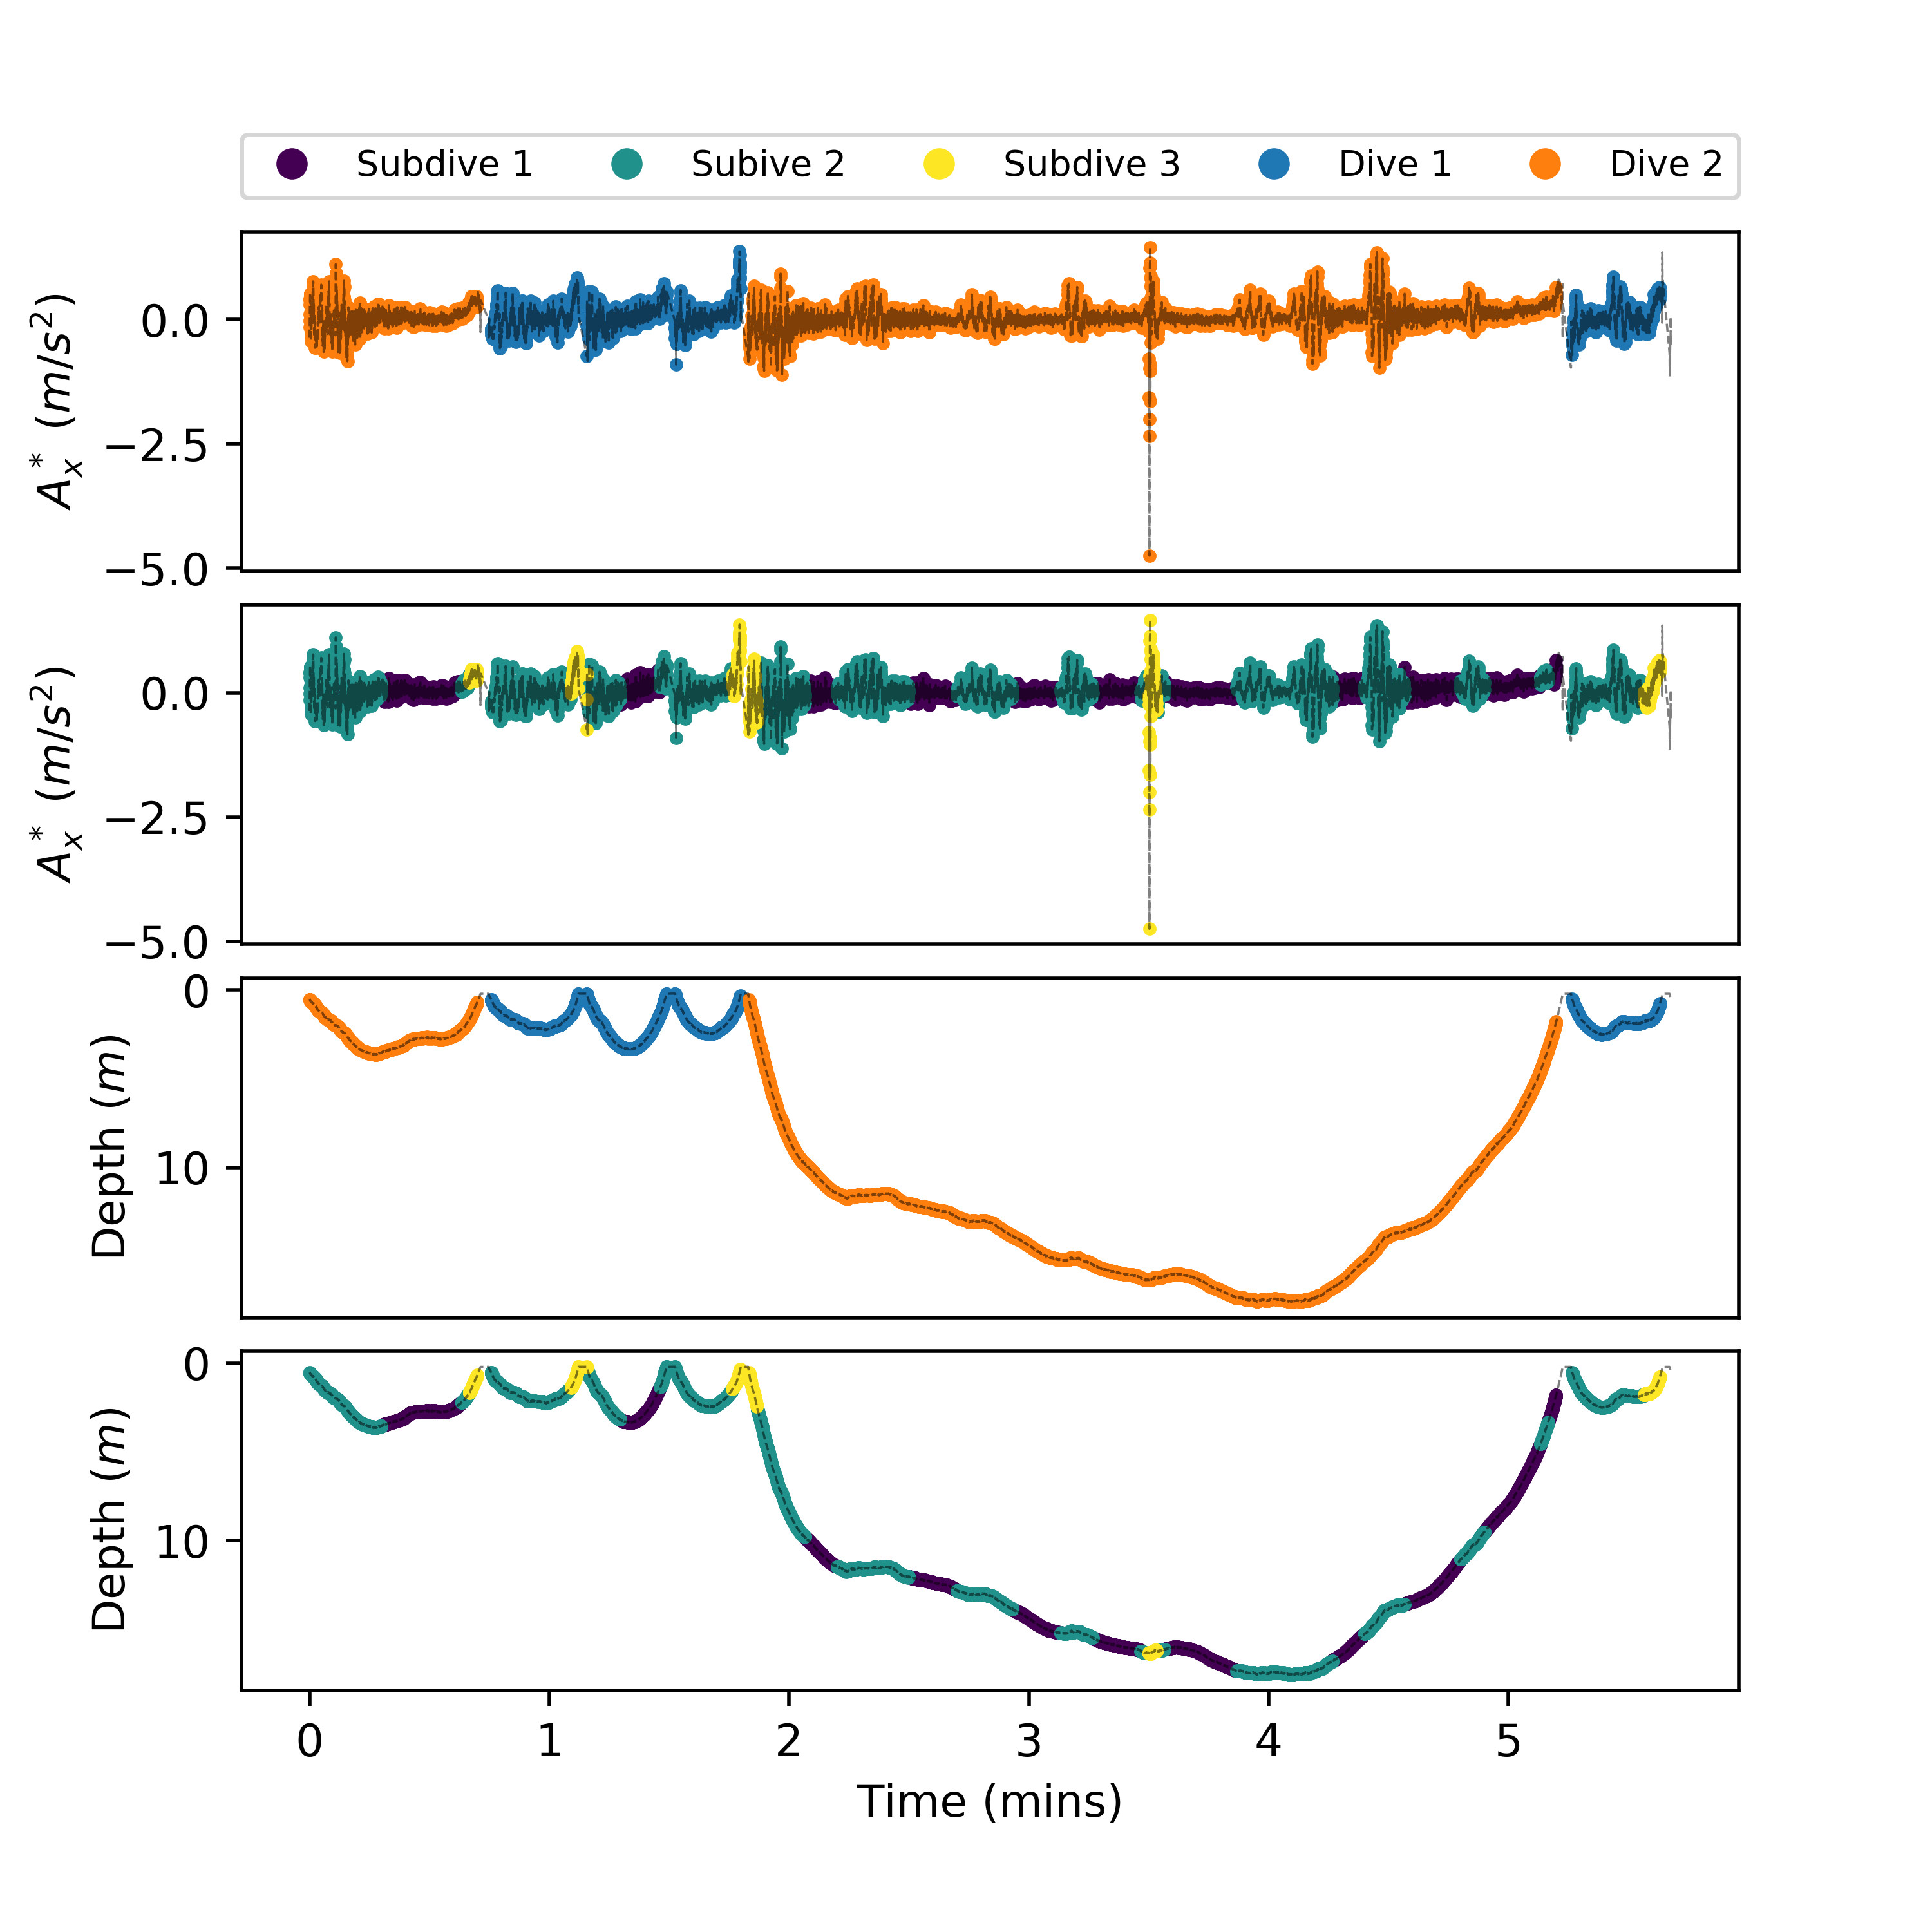
\includegraphics[width=5in]{../Plots/CarHHMM2_decoded_dives.png}
	\caption{Features of a particular set of killer whale dives and decoded estimates for the intra-dive behavioral states. The color of the plot corresponds to the behavioral or dive state with the highest probability.}
	\label{fig:labeled_dives}
\end{figure}

\begin{figure}[ht]
    \begin{subfigure}{0.45\textwidth}
    	\centering
    	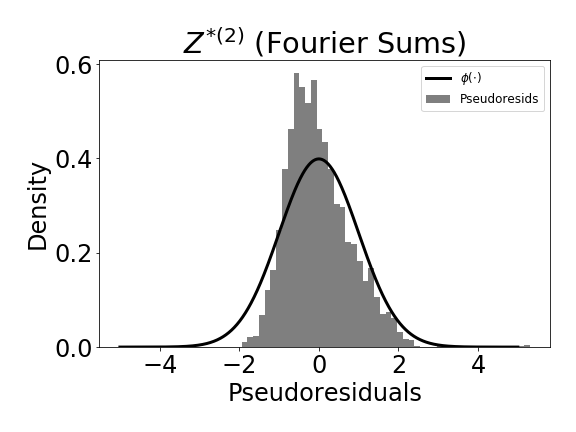
\includegraphics[width=2.25in]{../Plots/CarHHMM2_psedoresids_ahat.png}
    	\caption{Pseudoresiduals of $Z^{*(2)}$}
    	\label{fig:pseudoresids}
    \end{subfigure}
    \begin{subfigure}{0.45\textwidth}
    	\centering
    	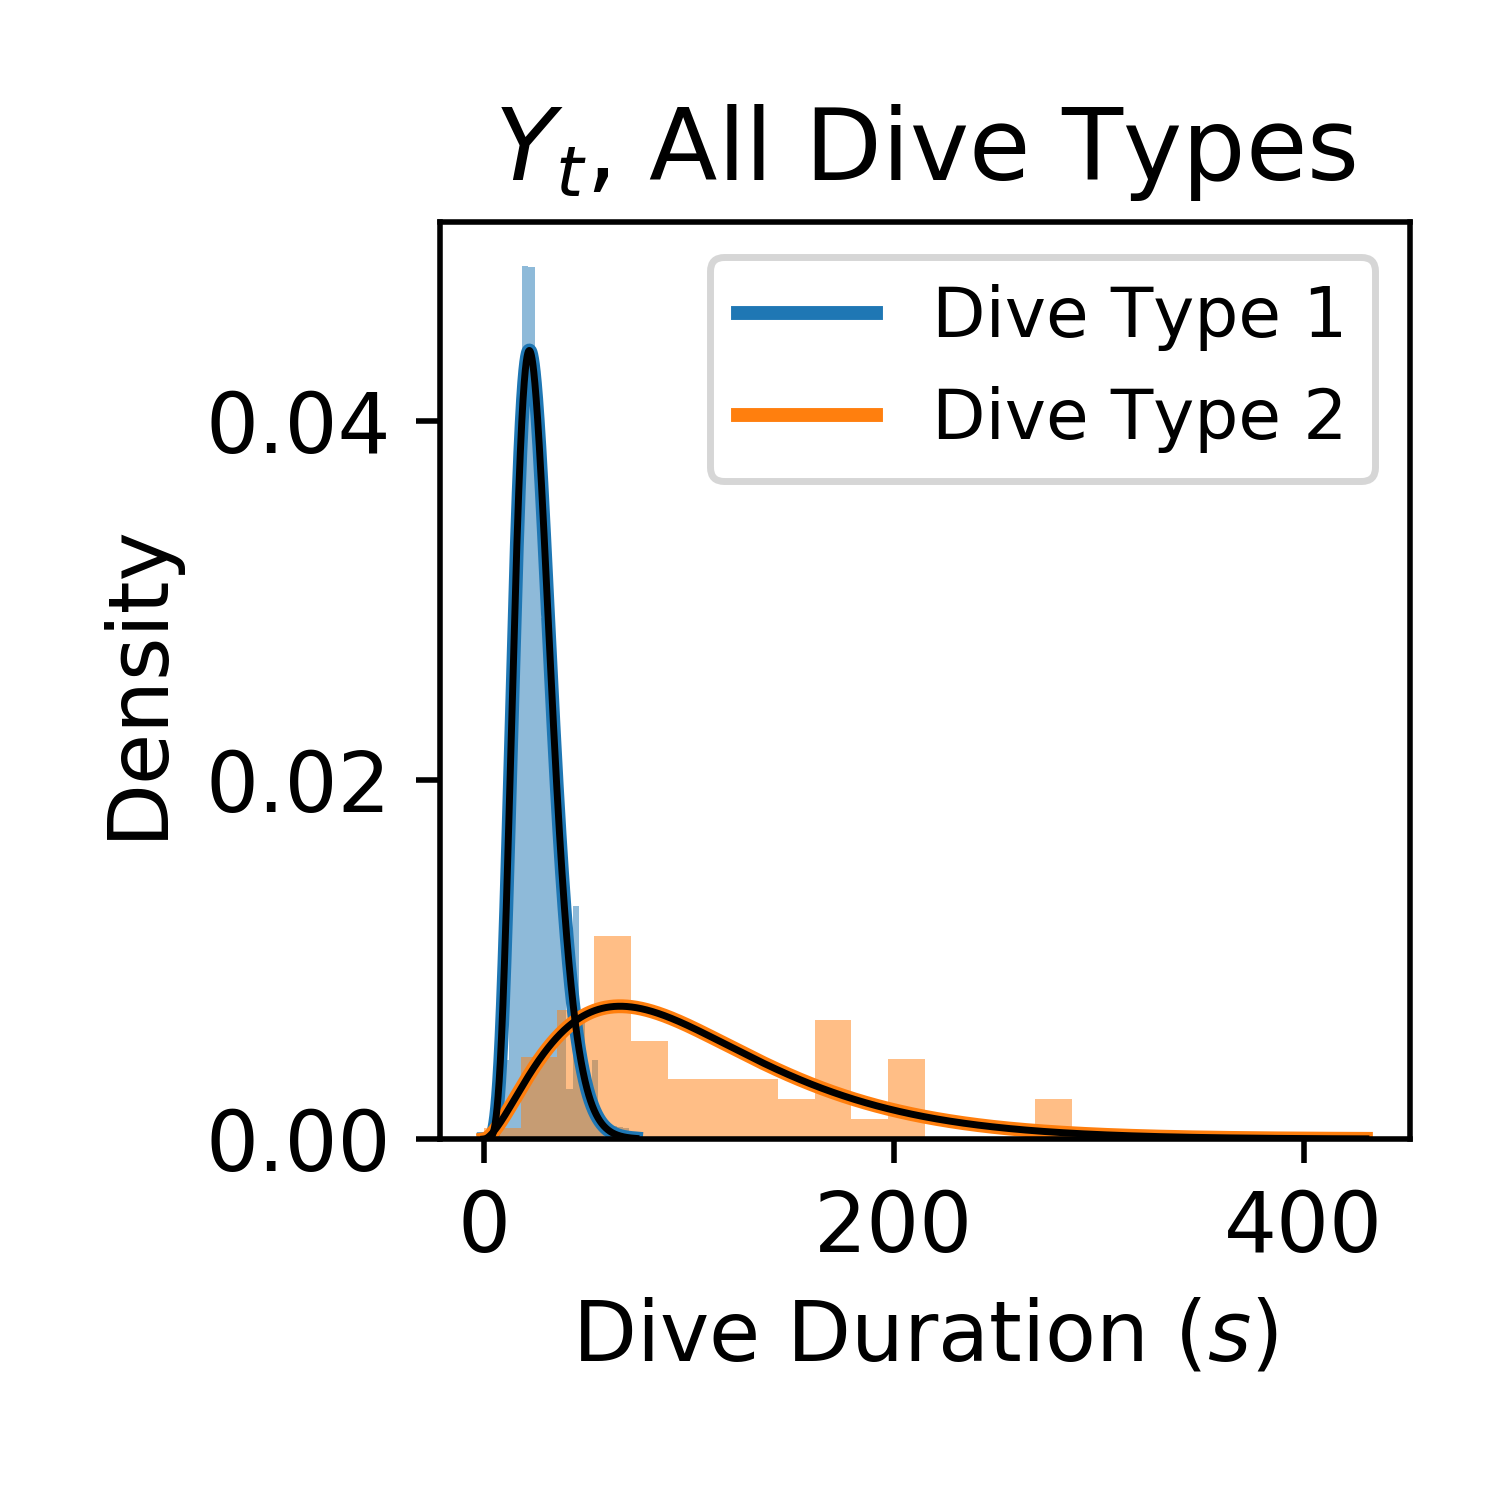
\includegraphics[width=2.25in]{../Plots/CarHHMM2_empirical_hist_dive_duration.png}
    	\caption{Empirical distribution of $Y$ (Dive Duration)}
    	\label{fig:empirical_dist}
    \end{subfigure}
    \caption{Examples of psuedoresiduals and a weighted empirical distribution as model checking tools}
    \label{fig:model_checking}
\end{figure}